\documentclass{report}

\usepackage{amsmath} % For math
\usepackage[english]{babel} % For hyphenation
\usepackage[backend=bibtex]{biblatex} % For bibliography
\usepackage{enumitem} % For lists spacing
\usepackage{fancyhdr} % For the fancy header
\usepackage{geometry} % For page margins
\usepackage{graphicx} % For images
\usepackage[hidelinks]{hyperref} % For links
\usepackage[utf8]{inputenc} % For input encoding
\usepackage{listings} % For source code embedding
\usepackage{setspace} % For line spacing
\usepackage{xcolor} % Syntax highlight for source code


% Bibliography
\addbibresource{bibliography.bib}
\addbibresource{sitography.bib}

% Code background
\definecolor{backgroundColour}{rgb}{0.95, 0.95, 0.96}

% C++ code style
\lstdefinestyle{CPPStyle} {
	language=C++,  
	basicstyle=\ttfamily,
	keywordstyle=\color{blue}\ttfamily,
	stringstyle=\color{red}\ttfamily,
	commentstyle=\color{magenta}\ttfamily,
	morecomment=[l][\color{magenta}]{\#},
    backgroundcolor=\color{backgroundColour},
    breakatwhitespace=false,
    breaklines=true,
    captionpos=b,
    keepspaces=true,
    showspaces=false,
    showstringspaces=false,
	showtabs=false,
	showlines=true,
	tabsize=4
}

% Page margins
\newgeometry{
    top=1.5in,
    bottom=1.5in,
    outer=1.5in,
    inner=1.5in,
}

% Page headers
\pagestyle{fancy}
\fancyhead[R]{{\nouppercase{\leftmark}}}
\fancyhead[L]{}

% Space between list elements
\setlist[itemize]{itemsep=1mm}


\title{Title}
\author{Michele Zoncheddu}
\date{March 2020}
\makeatletter

\begin{document}

\begin{titlepage}
	\centering
	
\includegraphics[height=12pc]{img/university_logos/cherubino_unipi.pdf}
	\bigbreak
	\bigbreak
	\bigbreak

	{\LARGE{\textbf{\@title}}}
	\bigbreak
	\bigbreak
	\medbreak

	{\large{Bachelor of Science Thesis}}
	\bigbreak
	\bigbreak
	\medbreak

	{\Large{\textbf{\@author}}}
	\bigbreak
	\bigbreak
	\medbreak

	{\Large{University of Pisa}}
	\bigbreak

	{\Large{Department of Computer Science}}
	\bigbreak

	{\Large{\@date}}
\end{titlepage}

\setstretch{1.15}
\tableofcontents
\setstretch{1.3}
\pagebreak

	\chapter{Introduction}
MoVEAS (acronym of Monitoring and Visualization of Early Autism Signs) is a project that aims to detect, in a non-invasive way, early signs of autistic spectrum disorders (ASD), by monitoring play activities in young children through sensorized toys and classifying the activities through a neural network \cite{Bon20, Lan19}.
\bigbreak

The way children interact with the world is called \textit{play} from adults. Observing children while playing is a widespread technique for diagnosing ASD, especially in early age \cite{Ozo08}, and videotaped play session of groups of children with typical development, against groups of children with ASD, have been proven to be useful for the diagnosis \cite{Bar05, Ozo08, Wet10}.

Children with ASD play in a differently from to their neurotypical peers: they use the toys in atypical and restricted ways (e.g. spinning), play with repetitive behaviors, and visually explore objects in unusual ways \cite{Bru07, Ozo08}.

Diagnosing ASD can be difficult, since there's no medical test to diagnose the disorders, and the \textit{spectrum width} makes it even harder. This project's aim is to simplify the specialists' diagnosis process, by identifying ASD-related behaviors and allowing to indirectly monitor the play session.
\bigbreak

This document will show how the development of the previous project has moved on, how the issues have been detected and solved, which features have been improved and which new ones have been added.

It will be illustrated the selection of the relevant data to classify the movements, the analysis of the consistency of the data obtained by the data fusion algorithms over time, then the comparison between two new neural network models, and the performance of the final model in a real scenario simulation.
\bigbreak

\paragraph{Thesis outline}
The next chapter describes the background for a better understanding of the rest of the thesis, such as theoretical concepts and practical details. Afterwards, it will be shown the previous version of the project' architecture, to introduce the actual development. Then, the achieved results are illustrated, and the final chapter summarizes the contributions of this work, putting forward suggestions for future developments.

	\newpage
	\chapter{Background}

\section{Hardware}
\subsection{Particle Photon}
Particle Photon is a tiny board (36.58mm $\times$ 20.32mm $\times$ 4.32mm in our configuration, weighing in at 5 grams) specifically designed for Internet of Things (IoT)\footnote{A system of typically embedded devices that connects to the Internet and to each other, without requiring human-to-human or human-to-computer interaction \cite{IoTAgenda}. There's still no baseline or standard definition, which is why IEEE is asking for suggestions to the community to provide it \cite{IEEEIoT}.} projects \cite{ParticlePhoton}, based on a relatively powerful but power efficient microcontroller of the STM32 ARM Cortex M3 family, with integrated Wi-Fi and the ability to interface itself with cloud services offered by Particle.

Unfortunately, the integrated Wi-Fi module has not been powerful enough to ensure a reliable connection in the tested scenarios, causing frequent disconnections. An Airgain's IPEX antenna, easily pluggable to the Photon through a U.FL connector, has allowed to achieve a more stable connection.
The code deployment can be performed seamlessly through a web-based IDE, that compiles and flashes the code to the selected device Over-The-Air (OTA). It is also possible to control the real-time device's status through a web-based console, that allows to flash the firmware to a specific version (downgrades are trickier than upgrades, especially OTA), and displays graphs for data such Wi-Fi's signal strength and quality, round trip time and memory usage.

\begin{center}
	\begin{figure}[ht!]
		\makebox[\textwidth]{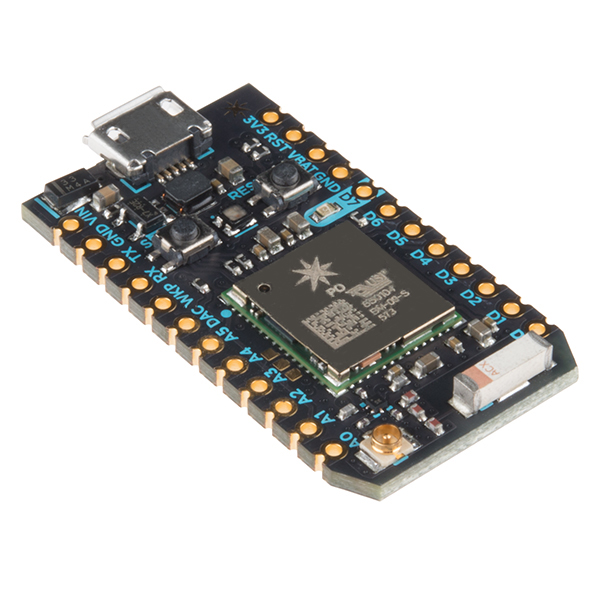
\includegraphics[width=0.3\paperwidth]{img/photon.jpg}}
		\caption{Particle Photon \cite{Photon}.}
	\end{figure}
\end{center}

\subsection{Sensors}
The SparkFun's sensor stick used in the project is a 9 Degrees of Freedom (9DoF) Magnetic, Angular Rate and Gravity (MARG) Micro-Electro-Mechanical Systems (MEMS) sensor. Its inertial module is the STMicroelectronics's LSM9DS1 integrated circuit, that features a digital linear acceleration sensor, a digital angular rate sensor and a digital magnetic sensor: each one can take measurements from $x$, $y$ and $z$ axes – hence 9 degrees of freedom.

The stick has been connected to the Photon through the I$^2$C serial bus interface. Its compact size and power efficiency make it ideal for embedded systems \cite{SensorDatasheet}.

\begin{center}
	\begin{figure}[ht!]
		\makebox[\textwidth]{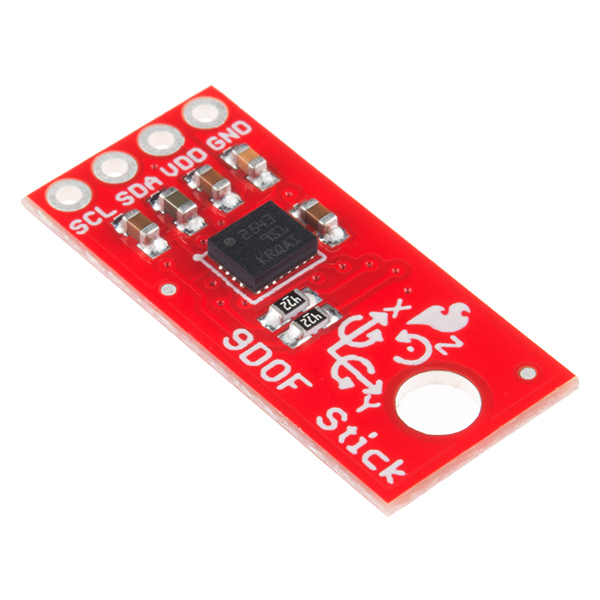
\includegraphics[width=0.3\paperwidth]{img/imu.jpg}}
		\caption{SparkFun Sensor Stick \cite{IMU}.}
	\end{figure}
\end{center}

\section{Software}

\subsection{Node.js}
Node.js is an open-source asynchronous event-driven JavaScript runtime environment that executes code outside of a browser, built on Google Chrome's V8 JavaScript engine \cite{Node.js}.

To put it simply, a synchronous execution environment needs to wait to one task to finish before moving to another; asynchronous execution, on the contrary, allows to move to another task before the previous one has finished. In a typically input/output (I/O) bound context, (like the network), for a single-threaded software (like Node.js) an asynchronous (non-blocking) I/O method allows to register the clients' requests, wait until the reply is available, and then call the related callback. This allows faster replies to the clients, compared to synchronous (blocking) I/O.

\subsection{Express.js}
Express.js, or simply Express, is a minimalist, open-source web framework for Node.js, designed for building web applications and APIs \cite{Express.js}. Its main feature is the routing mechanism: it allows to specify a callback function called when the application receives a request to the specified route and HTTP method. For example, using an Express \texttt{app} object, \texttt{app.get()} would handle GET requests, \texttt{app.post()} would handle POST ones, and so on.

\subsection{Three.js}
Three.js is a JavaScript library for creating animated 3D graphics in a web browser. Three.js uses WebGL (and simplifies its API) for creating GPU-accelerated 3D animations within web browsers without relying on proprietary plugins; in fact, Three.js is fully open-source.

\subsection{MQTT}
Message Queue Telemetry Transport (MQTT) is a machine-to-machine (M2M)/IoT connectivity protocol \cite{MQTT}. MQTT was designed as an extremely lightweight publish/subscribe messaging transport, and can be supported by any network protocol that provides ordered, lossless and bi-directional connections (typically TCP/IP) \cite{MQTTDoc}.

The MQTT protocol defines two types of network entities: a message broker (Mosca in the project) and a number of clients. An MQTT broker is a server that receives all messages from the clients and then routes the messages to the appropriate destination clients \cite{KnowMQTT}. An MQTT client is any device that runs an MQTT library and connects to an MQTT broker over a network \cite{ClientBroker}.

Information is organized in a hierarchy of topics. When a publisher has a new item of data to distribute, it sends a control message with the data to the connected broker. The broker then distributes the information to any clients that have subscribed to that topic. The publisher does not need to have any data on the number or locations of subscribers, and subscribers in turn do not have to be configured with any data about the publishers.

\subsection{MongoDB}
MongoDB is a general purpose, document-based, distributed database \cite{MongoDB}. Classified as a NoSQL database, it stores documents in a JSON-like format. MongoDB belongs to the category of document-oriented databases: the smallest unit of storage is a document; documents are stored in collections, which in turn make up a database. Documents are analogous to rows in a SQL table, but with one big difference: documents may have different structures. Another feature of MongoDB is that fields in a document can contain arrays and or sub-documents (sometimes called nested or embedded documents).

MongoDB stores data records as BSON documents. BSON is a binary representation of JSON documents, although it contains more data types than JSON \cite{BSONSpec}.

\subsection{TensorFlow and Keras}
TensorFlow is an open-source platform for machine learning developed by Google \cite{tensorflow15}. Since its first release, in 2015, has become the most popular deep learning framework \cite{Kha19}.

Its core is written in C++ and CUDA to achieve high performances, especially by using GPUs.
\bigbreak

Keras is an open source-library that works as API for neural networks frameworks, and it achieved so much popularity to became the official TensorFlow's frontend in 2017 \cite{WhyKeras}. Because it's written in Python, an higher level programming language with respect to C++, it's more intuitive to use instead of the TensorFlow raw functions.

\section{Rotation formalisms}
This section describes the mathematical formalisms to represent three-dimensional rotations in the project.

\subsection{Tait–Bryan angles}
Tait–Bryan angles (also called nautical angles or \textit{yaw, pitch and roll}) are a variant of Euler angles, normally used for aerospace applications (wherein they are often called Euler angles). Euler angles are a minimal representation (a set of three numbers) of relative orientation. This set of three angles describes a sequence of rotations about the axes of a reference frame. There are, however, sets that describe the same orientation: different combinations of $x$, $y$, and $z$ axes lead to different Euler angles \cite{Rob20}.

The only difference is that Tait–Bryan angles represent rotations about three distinct axes (e.g. $x$-$y$-$z$), while proper Euler angles use the same axis for both the first and third elemental rotations (e.g. $z$-$x$-$z$) \cite{Sta18}.

Once fixed a reference frame, \textit{yaw, pitch and roll} represent the rotation angle around the $z$, $y$, and $x$ axis, respectively.
If the rotation occurs about the axes of the original coordinate system, which remains motionless, the rotation is called \textit{extrinsic}, and when it occurs about the axes of the rotating coordinate system, which changes its orientation after each elemental rotation, the rotation is called \textit{intrinsic}. It's interesting to know that $z$-$y$-$x$ intrinsic rotations correspond to $x$-$y$-$z$ extrinsic ones, and the same applies to every reversed-order rotation.

\begin{center}
	\begin{figure}[ht!]
		\makebox[\textwidth]{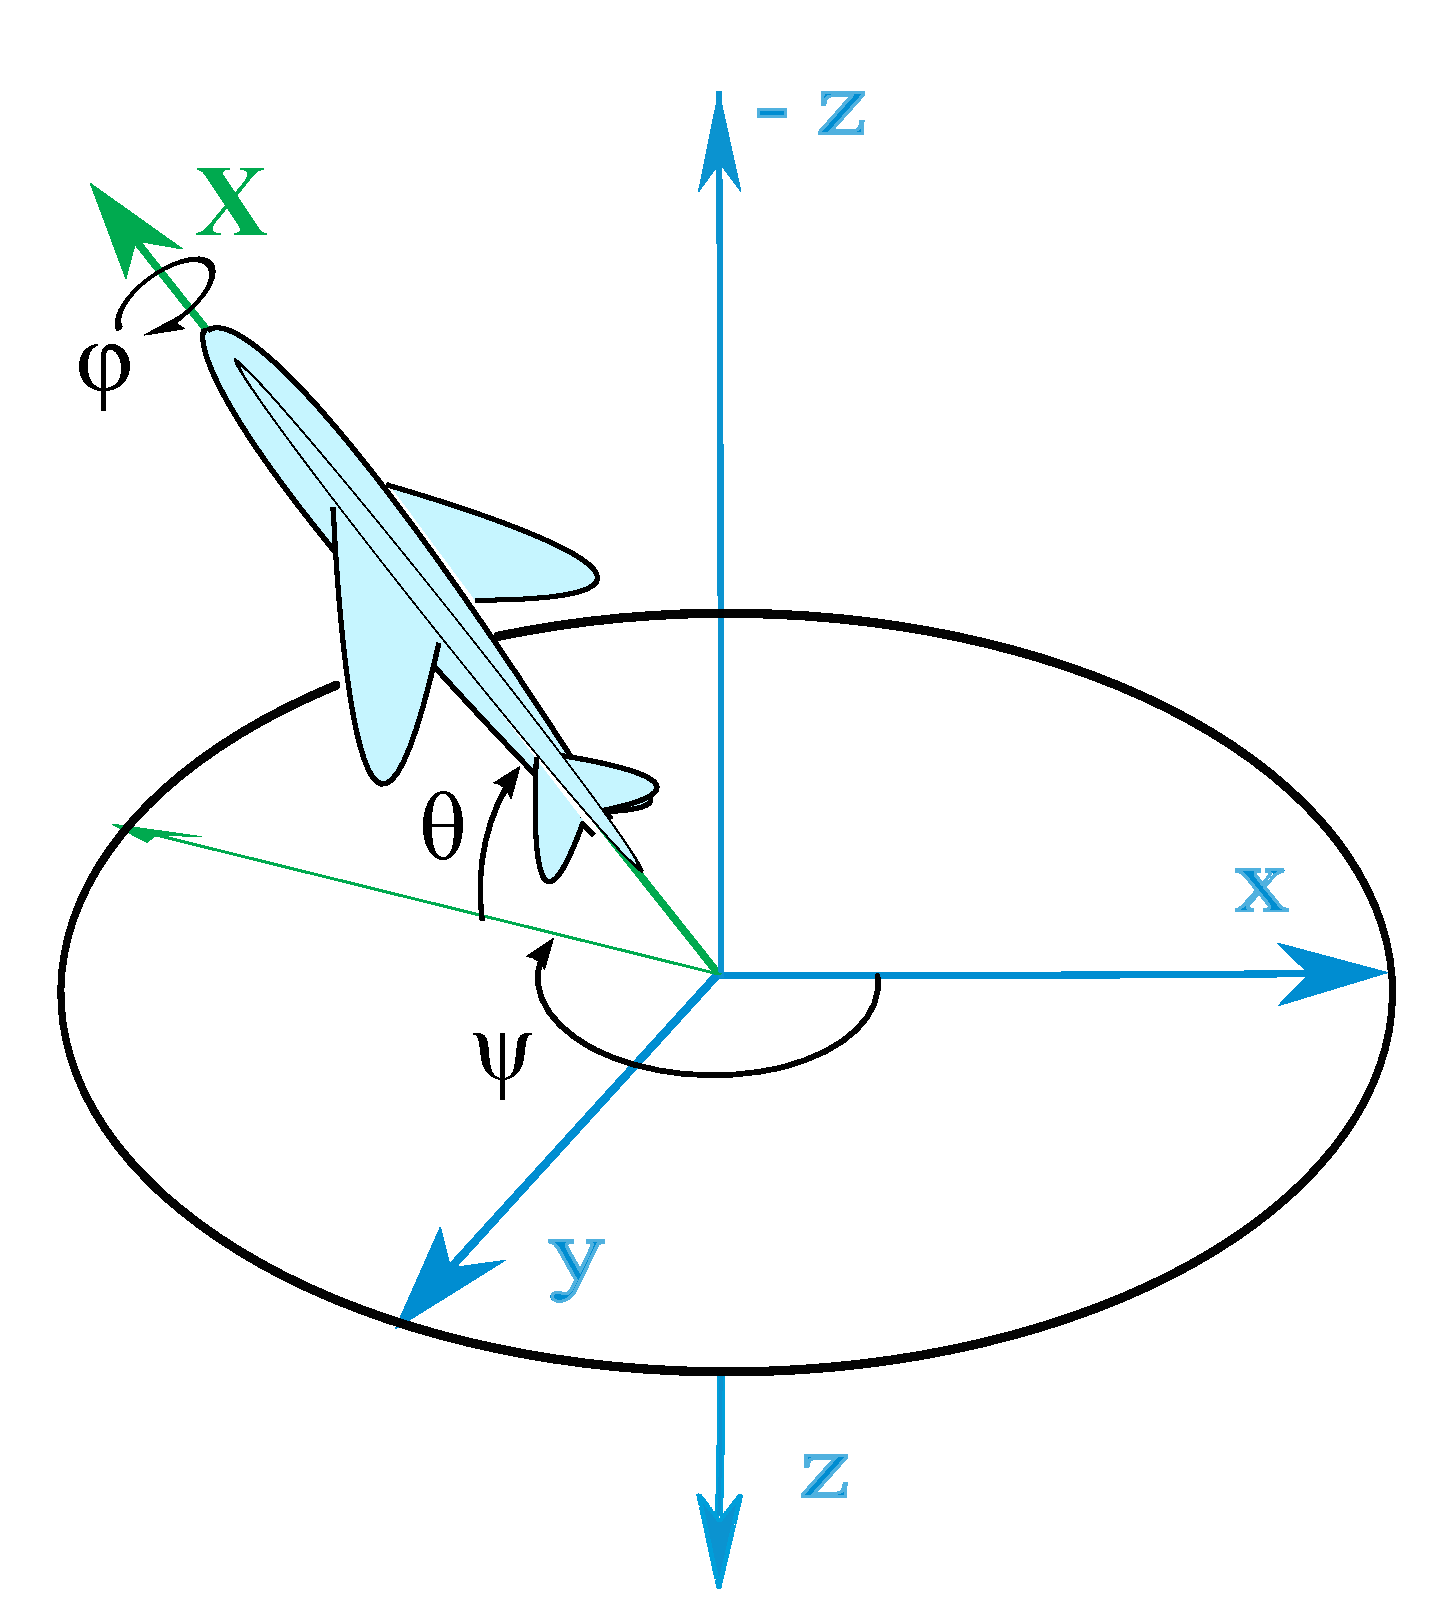
\includegraphics[width=0.35\paperwidth]{img/plane.pdf}}
		\caption{Yaw ($\psi$), pitch ($\theta$) and roll ($\varphi$) angles for an aircraft \cite{WikimediaPlane}.}
	\end{figure}
\end{center}
Representations with Euler angles share a problem called \textit{gimbal}\footnote{A \textit{gimbal} is a pivoted support that allows the rotation of an object about a single axis.} \textit{lock}\footnote{The word lock is misleading: no gimbal is restrained.}, that occurs when the orientation of the sensor cannot be uniquely represented, and causes a loss of a degree of freedom \cite{Dil18}.

An example: when the device pitches up 90$^{\circ}$ its pitch and yaw gimbals become aligned, and changes to roll and yaw apply the same rotation to the device \cite[68]{Tit04}.

This is a well-known problem for animating rotations, and it can be solved by adding a fourth gimbal actively driven by a motor so as to maintain a large angle between roll and yaw gimbal axes \cite{Bie99}, by mounting the inertial sensors directly to the body of the device (\textit{strapdown systems}) \cite[3]{Tit04}, or by representing rotations using quaternions instead of Euler angles.

\subsection{Quaternions}
Quaternions\footnote{Invented in 1843 by the famous mathematical physicist William Rowan Hamilton, they had been already described by Gauss in 1819, but his work was not published until 1900 \cite{Puj12}.} are four-dimensional entities that extend the complex numbers, and represent elements of $\mathbb{R}^4$ \cite{Ham47}. Compared to Euler angles, they are simpler to compose and avoid the problem of gimbal lock. Compared to rotation matrices, they are more compact, more numerically stable, and more efficient (more than twice as efficient as matrices on memory, and the quaternion multiplication is more than 1.5 times faster than matrix multiplication \cite{Gol10}).

As it represents an element of $\mathbb{R}^4$, a quaternion can be written as:

\begin{center}
	$q = (q_0, q_1, q_2, q_3)$
\end{center}
where $q_0$, $q_1$, $q_2$, and $q_3$ are real numbers, but it is generally represented this way:

\begin{center}
	$\textbf{q} = q_0 + \textbf{i}q_1 + \textbf{j}q_2 + \textbf{k}q_3$
\end{center}
where \textbf{i}, \textbf{j} and \textbf{k} are the standard orthonormal basis in $\mathbb{R}^3$ \cite{Kui99}; it always follows the fundamental formula of quaternion algebra:

\begin{center}
	$\textbf{i}^2 = \textbf{j}^2 = \textbf{k}^2 = \textbf{ijk} = -1$
\end{center}
Quaternions have a fundamental role in the project, since the Madgwick filter \cite{Mad10} and the 3D representation through Three.js heavily rely on them.

Algebra behind quaternions rotations will not be treated, because its complexity doesn't allow to simplify the main concepts in few lines; however, it can be found in \cite[127-134]{Kui99}.

\subsection{Rotation matrix}
In two dimensions, a rotation matrix $R \in \mathbb R^{2 \times 2}$ is a matrix that is used to perform a rotation in Euclidean space. Given a vector $\vec u \in \mathbb R^2$ and an angle $\theta \in \mathbb R$, the vector $\vec u$ rotated through an angle $\theta$ can be written as $R(\theta) \vec u$.

The matrix

\[
	R =
	{\begin{pmatrix}
		\cos \theta & -\sin \theta \\
		\sin \theta & \cos \theta
	\end{pmatrix}}
\]
rotates points in the $xy$-plane counterclockwise in a \textit{right-handed coordinate system} ($y$ counterclockwise from $x$) through an angle $\theta$ with respect to the $x$ axis about the origin of a two-dimensional Cartesian coordinate system. To perform the rotation of a point $p$ with coordinates ($x$, $y$), it should be written as column vector, and multiplied by the matrix $R$:

\[
	p_{rotated} = Rp =
	{\begin{pmatrix}
		\cos \theta &-\sin \theta \\
		\sin \theta &\cos \theta
	\end{pmatrix}}
	\cdot
	{\begin{pmatrix}
		x \\
		y
	\end{pmatrix}} =
	{\begin{pmatrix}
		x\cos \theta -y\sin \theta \\
		x\sin \theta +y\cos \theta
	\end{pmatrix}}
\]
How to represent \textit{yaw, pitch and roll}?\\
A \textit{yaw} is a counterclockwise (CCW) rotation of $\alpha$ on the $z$-axis. The rotation matrix is
\[
	R_z(\alpha) =
	\begin{pmatrix}
		\cos\alpha & -\sin\alpha & 0 \\
		\sin\alpha & \cos\alpha & 0 \\
		0 & 0 & 1
	\end{pmatrix}
\]
Note that the upper left values compose a 2D rotation matrix, and the coordinates on the third dimension (around whom the rotation happens) are left unchanged. The same applies to the other two matrices, but with the second and the first dimension.\\
A \textit{pitch} is a CCW rotation of $\beta$ on the $y$-axis. The rotation matrix is
\[
	R_y(\beta) =
	\begin{pmatrix}
		\cos\beta & 0 & \sin\beta \\
		0 & 1 & 0 \\
		-sin\beta & 0 & \cos\beta
	\end{pmatrix}
\]
A \textit{roll} is a CCW rotation of $\gamma$ on the $x$-axis. The rotation matrix is
\[
	R_x(\gamma) =
	\begin{pmatrix}
		1 & 0 & 0 \\
		0 & \cos\gamma & -\sin\gamma \\
		0 & sin\gamma & \cos\gamma
	\end{pmatrix}
\]
The final rotation matrix is obtained by the multiplication of the previous three:
\begin{gather*}
	R(\alpha, \beta, \gamma) = R_z(\alpha) R_y(\beta) R_x(\gamma) = \\
	\begin{pmatrix}
		\cos\alpha \cos\beta & \cos\alpha \sin\beta \sin\gamma - \sin\alpha \cos\gamma & \cos\alpha \sin\beta \cos\gamma + \sin\alpha \sin\gamma \\
		\sin\alpha \cos\beta & \sin\alpha \sin\beta \sin\gamma + \cos\alpha \cos\gamma & \sin\alpha \sin\beta \cos\gamma - \cos\alpha \sin\gamma \\
		-\sin\beta & \cos\beta \sin\gamma & \cos\beta \cos\gamma
	\end{pmatrix}
\end{gather*}
It is important to note that $R(\alpha, \beta, \gamma)$ performs the roll first, then the pitch, and finally the yaw. If the order of these operations is changed, a different rotation matrix results \cite{Lav06}.

Given an acceleration vector $\vec a$, the rotated one is obtained by the matrix-vector multiplication

\[
	\vec a_r = R(\alpha, \beta, \gamma) \vec a
\]

\subsection{Spherical coordinates}
Spherical coordinates specify the position of a point in a three-dimensional space using three numbers: $\rho$, $\theta$ and $\phi$, where $\rho$ represents the radial distance of the point from the origin, $\theta$ represents the angle of the the $z$-axis with the line that represents the distance, and $\phi$ represents the angle between the $x$-axis and the projection of the point on the plane generated by the $xy$-axes \cite{Sok}.

\begin{center}
	\begin{figure}[ht!]
		\makebox[\textwidth]{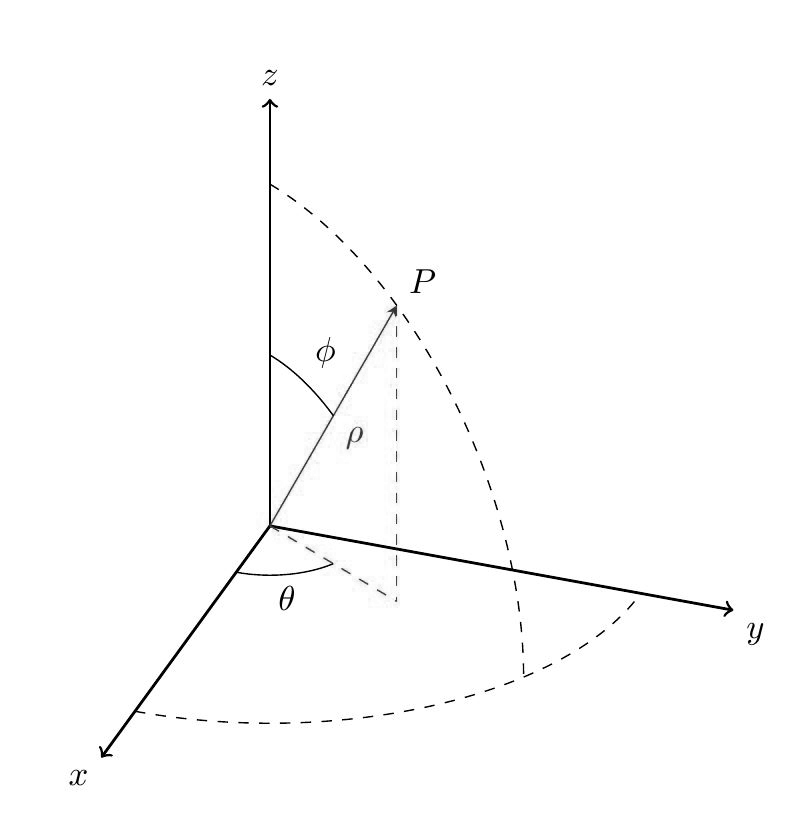
\includegraphics[width=0.45\paperwidth]{img/spherical_acc.jpg}}
		\caption{Spherical coordinates of the point P \cite{HartleySpherical}.}
	\end{figure}
\end{center}
The spherical coordinates are related to the Cartesian ones ($x$, $y$ and $z$) by the formulas \cite{Sok}

\[
	x = \rho \cos\phi \sin\theta \quad\quad y = \rho \sin\phi \sin\theta \quad\quad  z = \rho \cos\theta
\]
where the typical constraints

\[
	0 \leq \rho < \infty \quad\quad 0 \leq \phi < 2\pi \quad\quad 0 \leq \theta \leq \pi
\]
ensure an unique representation.

\section{Filters}
Motion representation can be obtained through accelerometer reading within the $x$, $y$ and $z$ axes, that make up an acceleration vector.

MEMS sensors are known to be very noisy, especially when working at high reading frequencies \cite[7]{Mat08}, and the noise is of a specific type, the Additive White\footnote{White noise is a random signal with constant amplitude across the whole frequency spectrum \cite{Feh97}.} Gaussian\footnote{Noise with a probability density function equal to that of the normal distribution, which is also known as the Gaussian distribution \cite{Feh97}.} Noise (AWGN) \cite{Yas03}. An effective way to remove AWGN is to use the Kalman filter \cite{Ko07, Sär15}, as it assumes that the errors are Gaussian \cite{Kal60}.

\subsection{Kalman filter}
Kalman filtering, also known as linear quadratic estimation (LQE) \cite{Ma19}, is an efficient recursive algorithm that uses a series of measurements observed over time, containing statistical noise and other inaccuracies, and produces estimates of unknown variables (the internal state of a linear dynamic system\footnote{Linear dynamic systems are systems in which its evolution is described by a linear function and hence satisfies the superposition principle.} \cite[47]{Ma19}) \cite[7-8]{Ma19}. This approach tends to be more precise than those based on a single measurement alone, because it uses using Bayesian inference and estimates a joint probability distribution over the variables for each timeframe \cite[8]{Ma19}.

Kalman filter is most often conceptualized as two distinct phases \cite[12-13]{Ma19}:

\begin{itemize}
	\item time updating: prediction phase, where the previous timesteps are used to predict the current one's state (\textit{a priori} state estimate);
	\item measure update: observation phase, where the prediction is combined with the current observation information to refine the state estimate (\textit{a posteriori} state estimate).
\end{itemize}

The Kalman filter has numerous applications in technology, like navigation and control of vehicles, particularly aircraft, spacecraft (NASA) and dynamically positioned ships \cite{Tri83, Fun83}.

\subsection{Madgwick filter} \label{Madgwick filter}
In 2009 Sebastian O. H. Madgwick, as part of his Ph.D research at the University of Bristol, developed an orientation filter for IMU (6DoF: tri-axis gyroscope and accelerometer) and MARG (9DoF: IMU + tri-axis magnetometer) sensors.

The filter is based on an optimized gradient-descent algorithm that fuses together the \textit{raw} data from the sensors \cite{Mad10}, and uses an analytically derived Jacobian matrix\footnote{A matrix of partial derivatives of a function.} to find a quaternion that minimizes the estimation's error \cite{Che12}.
\bigbreak

There are three interesting features \cite{Mad10}:
\begin{itemize}
	\item it is computationally inexpensive, thanks to the quaternion representation of rotation;
	\item it is effective at relatively low sampling rates, e.g. 10 Hertz. This is a big advantage, because Kalman-based filters may require sampling rates that exceed the bandwidth;
	\item its parameters can be changed according to the usage environment characteristics.
\end{itemize}

The low computational load reduces the hardware and power necessary for inertial movement tracking, allowing to create lightweight and inexpensive systems, capable of functioning for extended periods of time \cite{Mad11}.

\section{Neural networks}
Machine learning is a subfield of computer science that studies algorithms and statistical models to construct computer programs that automatically improve with experience \cite{Mit97}. Machines don't really learn\footnote{The name ``machine learning'' was coined by Arthur Samuel in 1959, while working for IBM on computers that learned how to play checkers when given only the rules of the game \cite{Sam59}.}, but typically build a mathematical function that produces the desired output when applied to a collection of inputs, called \textit{training data}, and this function is used to make predictions on inputs not encountered during training. The ability to make accurate predictions on new data is called \textit{generalization} \cite{Hay08}.
\bigbreak

There are two kinds of ``learning'' processes:
\begin{itemize}
	\item \textit{supervised}, when the training data is labeled or classified with the correct answer, and the network can use it to improve its performance. The goal is to minimize a loss function, which quantifies the training error; the networks are most often trained with the \textit{backpropagation}, a gradient-descent algorithm that computes the gradient of the loss function, to change them accordingly to the training;
	\item \textit{unsupervised}, when the training data is neither labeled or classified, and the network has to find by itself the way to categorize the data. In this case, the performance measurement is task-independent \cite{Hay08}.
\end{itemize}
One of the most famous statistical model for machine learning is the artificial neural network, commonly referred as ``neural network''. It's composed of multiple layers of inter-connected nodes. The term \textit{neural} suggest the parallelism with the biological neural networks that form animal brains, since the Rosenblatt's \textit{perceptron}\footnote{After the McCulloch and Pitt’s neuron, the perceptron was the next step towards the neural networks.} was born to mimic certain part of the neuron, such as dendrites, that receive the electrochemical stimulation from other neural cells, and axons, that propagates it.

The building block of the neural networks is the \textit{neuron}, an information-processing unit that works in this way: takes the inputs from weighted links, adds the weighted input signals together, and finally uses the sum as an input for the activation function; this function's output can be an input for another neuron, or part of the network's output.

\begin{center}
	\begin{figure}[ht!]
		\makebox[\textwidth]{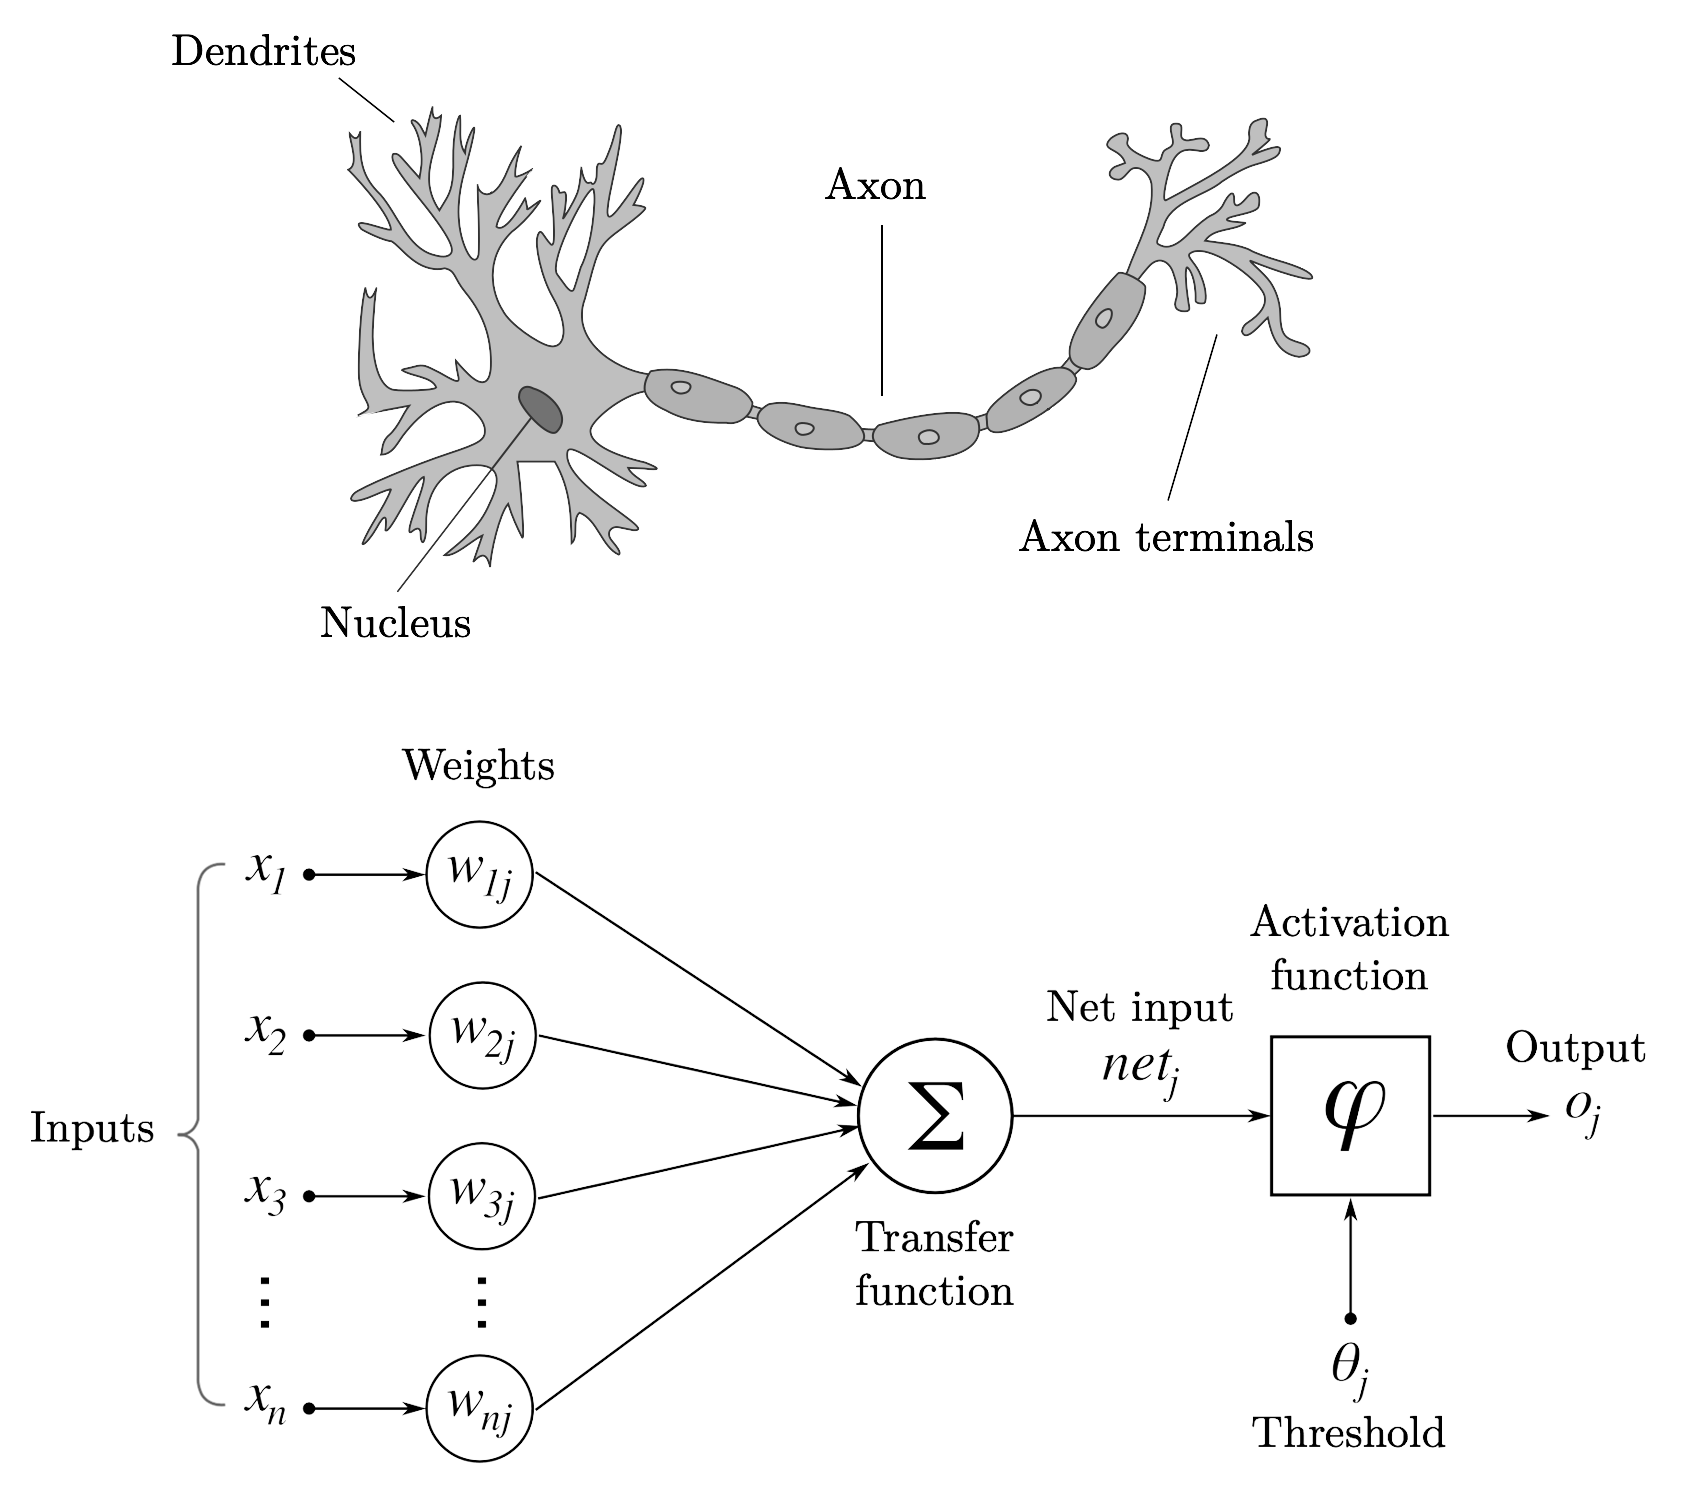
\includegraphics[width=0.65\paperwidth]{img/artificial_biological_network.png}}
		\caption{Similarities between biological \cite{WikipediaNeuron} and artificial neurons.}
	\end{figure}
\end{center}
There are three fundamentally different classes of network architectures \cite{Hay08}:

\begin{itemize}
	\item \textbf{single-layer feedforward networks}: in a layered network, the neurons are organized in form of layers, and in this case, the first layer of nodes, also called \textit{input layer}, feeds its output directly to the last (second) layer, called \textit{output layer}, where the neurons perform the computation. These networks are called \textit{feedforward} because the information moves in only one direction, forward, from the input nodes to the output ones;
	\item \textbf{multi-layer feedforward networks}: in this model, between the input and the output layer, there are one or more \textit{hidden layers} of neurons. The term ``hidden'' refers to the fact they're not seen directly from either the input or output of the network. By adding hidden layers, the network is capable to extract higher-order statistics from its input;
	\item \textbf{recurrent networks}: differently from feedforward neural networks, in this architecture there is at least one feedback loop. Feedforward neural network remember what they learnt during training, while recurrent ones, in addition, remember things learnt from previous inputs while generating outputs. Along with the fact that this model can deal with variable length inputs, makes them applicable to time-dependent tasks, like weather forecasting or speech recognition.
\end{itemize}

\begin{center}
	\begin{figure}[ht!]
		\makebox[\textwidth]{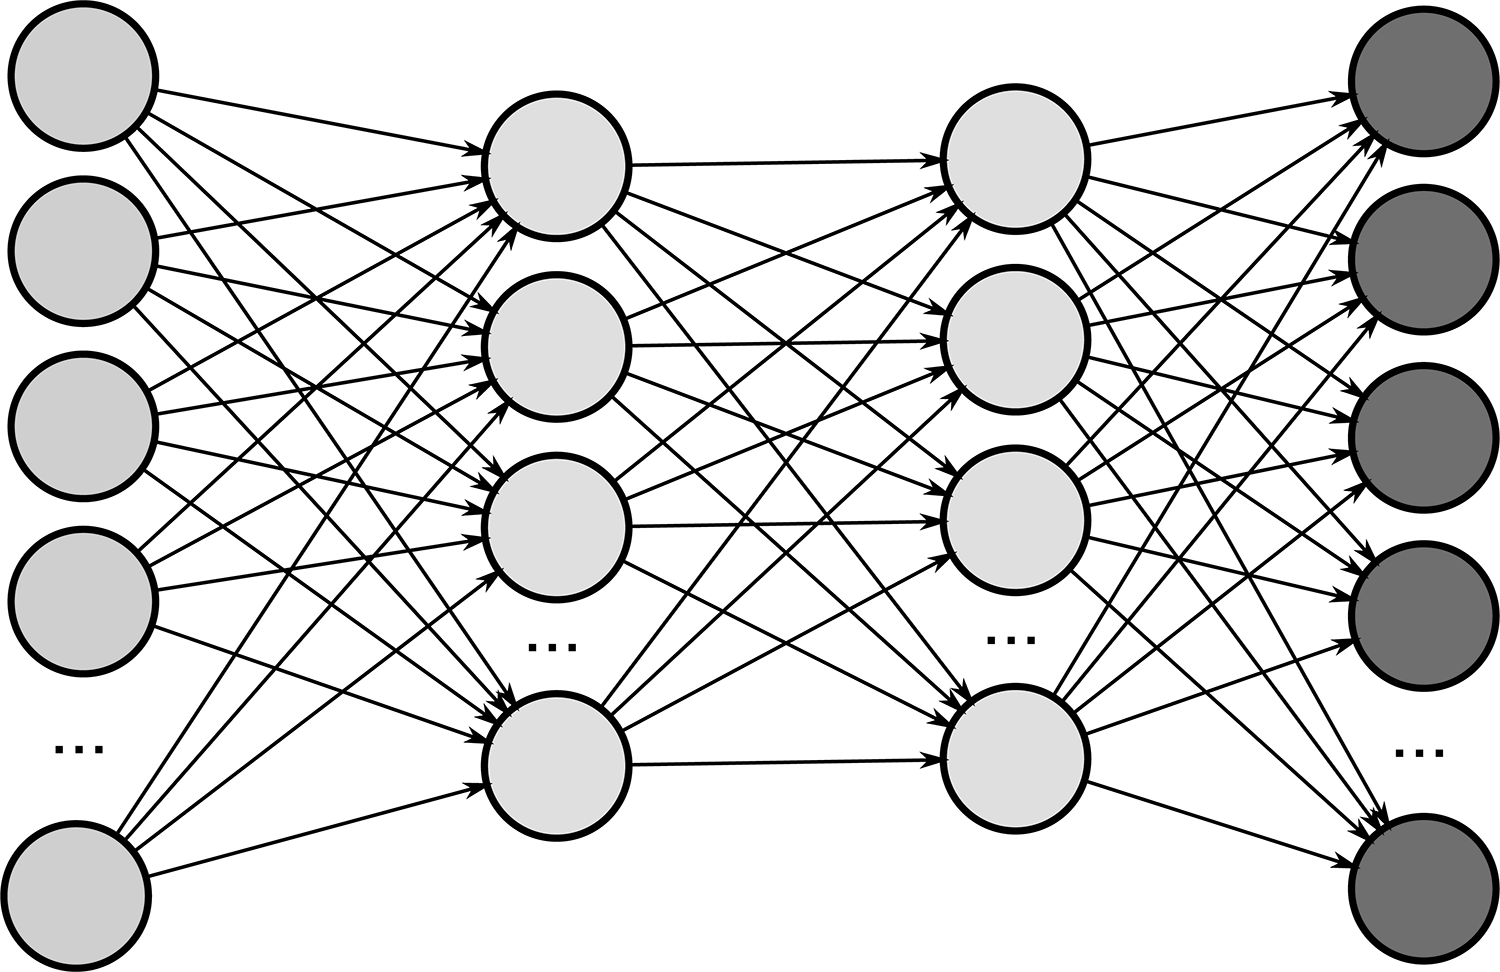
\includegraphics[width=0.4\paperwidth]{img/neural_network.png}}
		\caption{A fully-connected feedforward neural network with two hidden layers.}
	\end{figure}
\end{center}

\subsection{Time delay neural networks}
Time delay neural network (TDNN) is one of the simplest neural network that provides \textit{shift-invariant} pattern classification. \textit{Shift-invariance} means that different displacements of the features in the pattern don't affect the prediction. TDNNs were invented in 1989 to classify phonemes in speech signals for automatic speech recognition; the fact that the TDNN recognizes phonemes independently of their position in time, significantly improved the performance over static classification \cite{Wai89}.
\bigbreak

TDNNs are most often implemented by the machine learning frameworks with 1-dimensional convolutional neural network (CNN).\\
2-dimensional CNNs are widely used for image classification, where the two dimensions are the $x$ and the $y$ axis; in time series classification, of course, the only dimension is the time.
\bigbreak

Convolution is a linear mathematical operator defined as the integral of the product of two functions, that produces a third function; CNNs use convolution in place of general matrix multiplication \cite{Goo16}. The convolution is defined as:

\[
	(f*g)(t)\,
		\triangleq
	\int_{-\infty }^{\infty} f(\tau)g(t-\tau)\, d\tau\,
		=
	\int_{-\infty }^{\infty} f(t-\tau)g(\tau)\, d\tau
\]
\newline
In CNNs, there are two types of layers:
\begin{itemize}
	\item the \textit{convolutional layer}, that through a fixed-size window, called \textit{kernel}, slides over the inputs and gives its outputs to the next layer. The kernel of \textit{filters} computes the dot product between its weights and the inputs (this process is called \textit{convolution}), and projects the output in a n-dimensional space, where n is the number of output filters in the convolution;
	\item the \textit{pooling layer}, that takes the maximum value of the input's patch (max-pooling) or the average (average-pooling), or other values by using different approaches, performing a down-sampling.
\end{itemize} 
The \textit{shift-invariance} is provided by the kernel's \textit{weights sharing}, that means that the same weights are used across the entire layer's input, so they will learn independently of their position. The kernel's shift over the input after every step is called \textit{stride}, and it's typically 1, but it can be higher to perform down-sampling.
\bigbreak

\begin{center}
	\begin{figure}[ht!]
		\makebox[\textwidth]{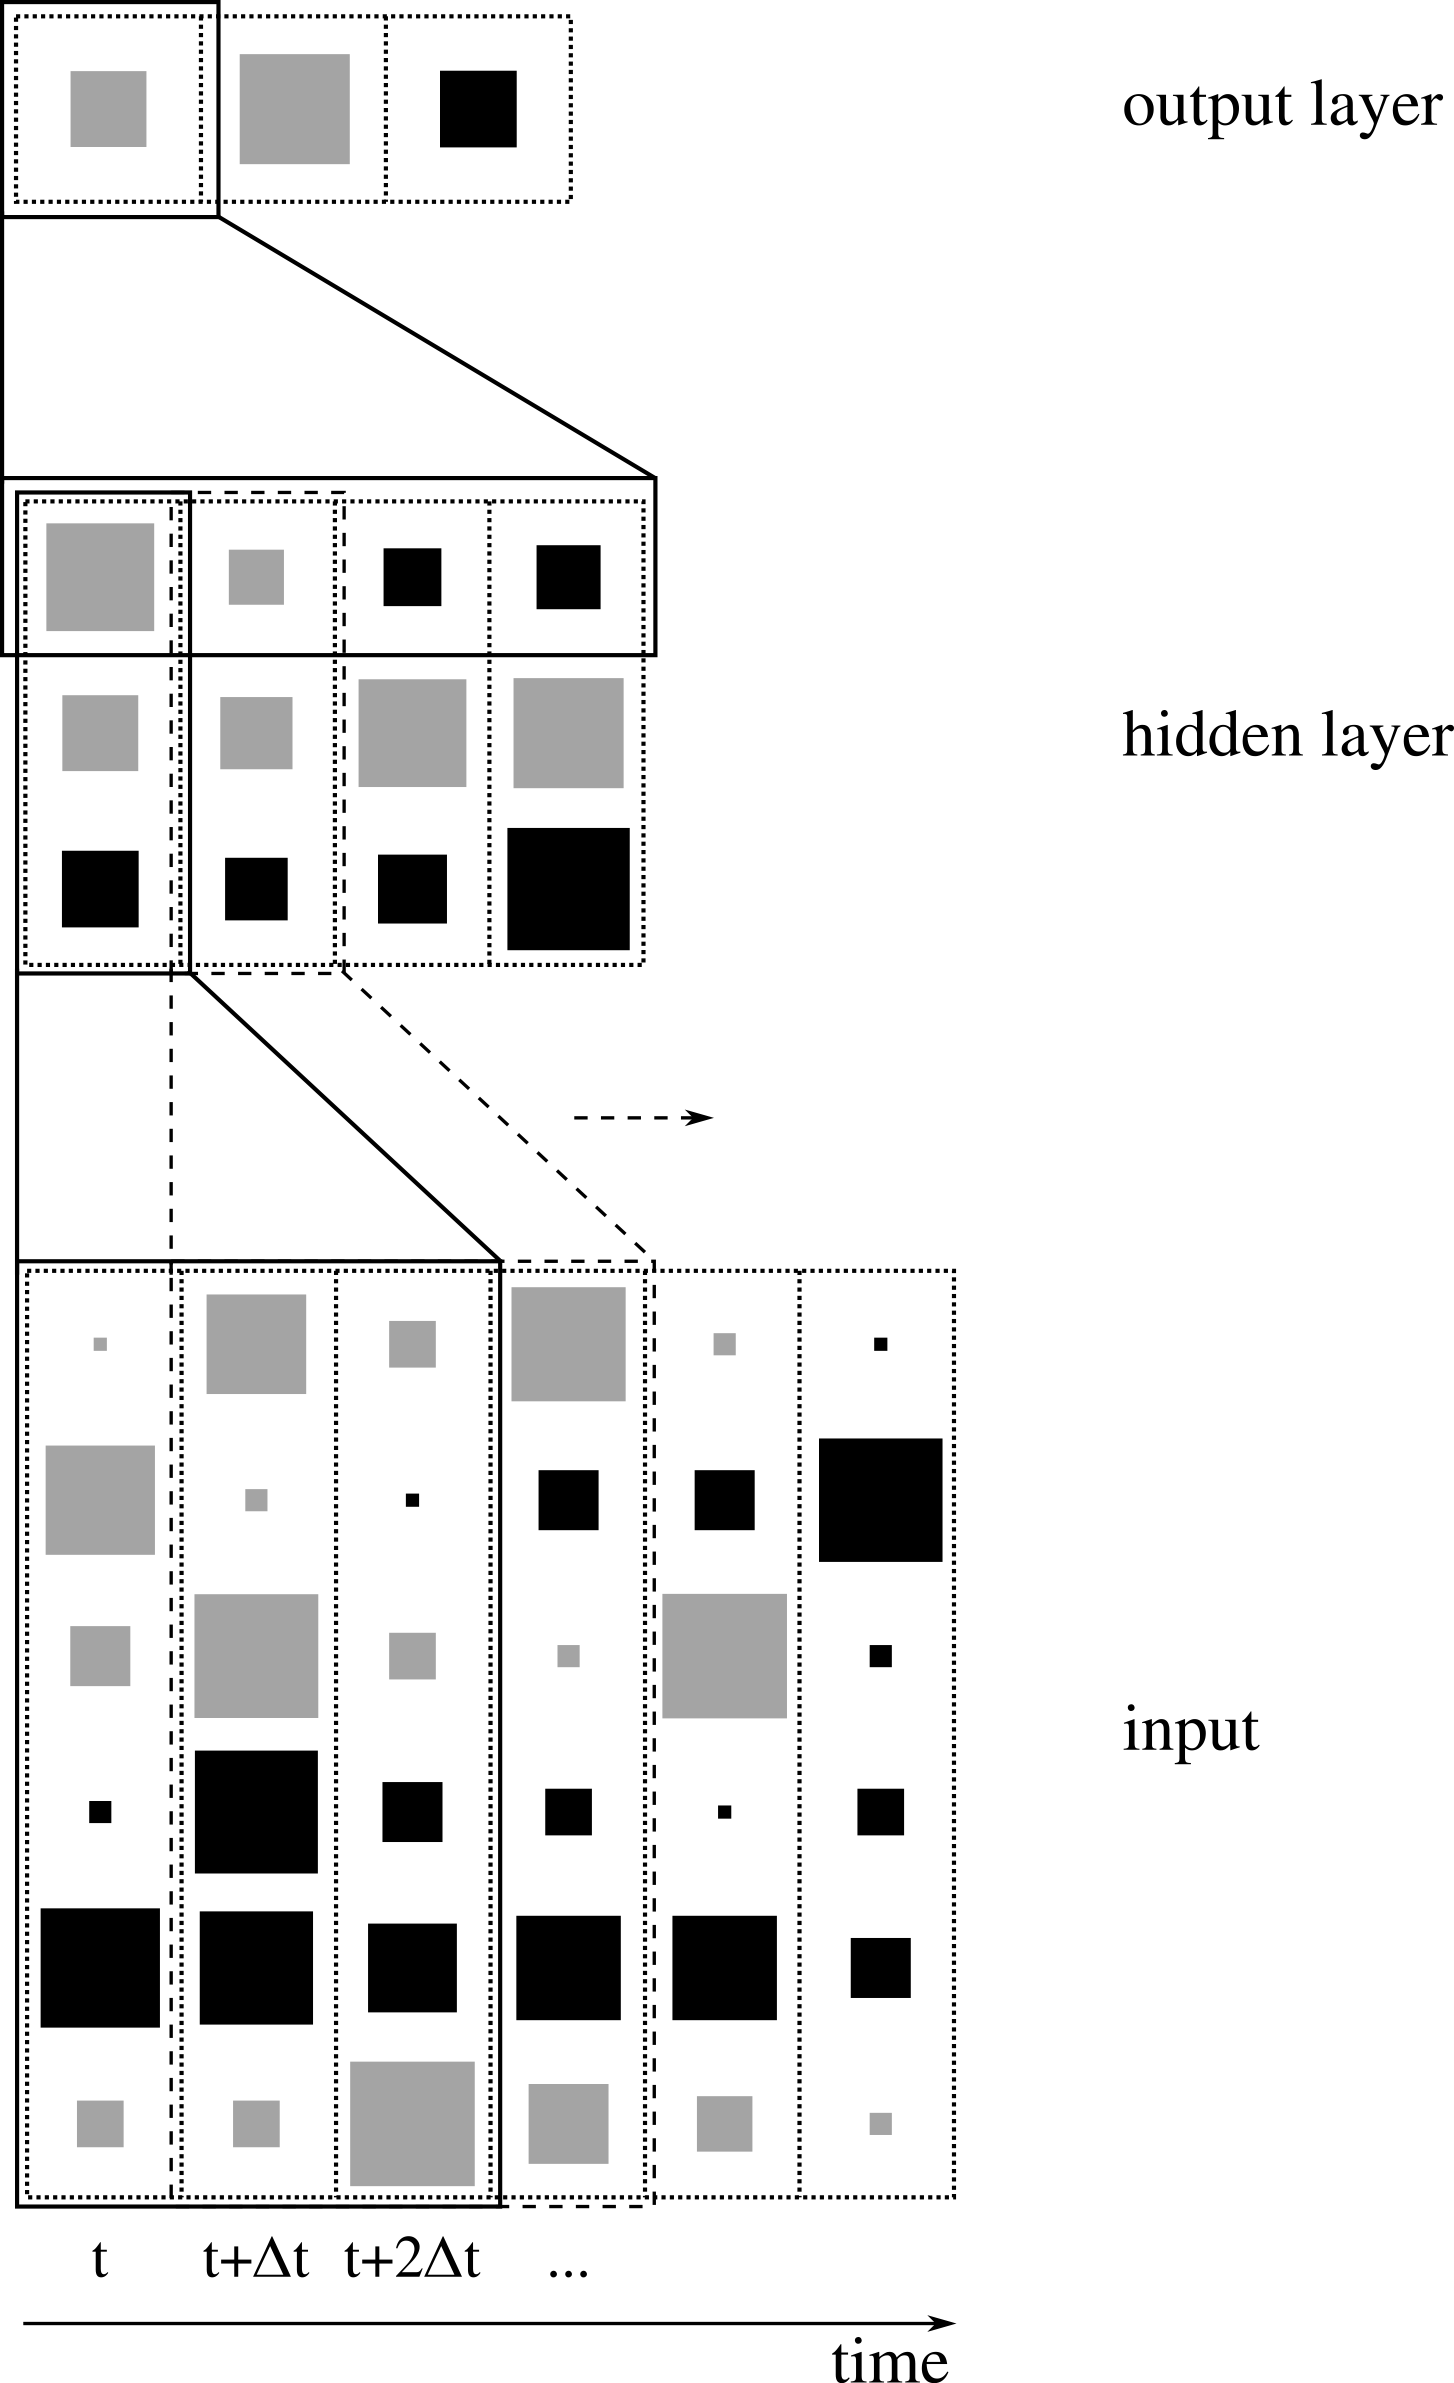
\includegraphics[width=0.3\paperwidth]{img/tdnn.png}}
		\caption{TDNN diagram \cite{WikipediaTDNN}.}
	\end{figure}
\end{center}

\subsection{Recurrent neural networks}
Recurrent neural networks (RNN) are networks in which there is at least one \textit{feedback loop}. The presence of loops and self-loops connections provides the network dynamical properties, leaving a memory (states) of the past computations in the model, and allowing it to process variable-length inputs \cite{Yan09} (it's like a new layer is created for each encoding step of the input sequence). This makes them ideal for handwriting recognition or speech recognition \cite{Gra09, Li15}.
\bigbreak

The most common learning algorithm is a generalization of the backpropagation for feedforward neural networks, and it's based on unfolding the recurrent network' states in time: it's called \textit{backpropagation through time} (BPTT) \cite{Wer88}.
\bigbreak

A famous RNN model is the long short-term memory (LSTM), that allowed to solve the \textit{vanishing gradient problem} (through BPTT), that especially affected RNN when unfolding deep layers \cite{Pas12}.

This model also revolutionized handwriting recognition \cite{Fer07, Gra09}, speech recognition \cite{Li15}, text-to-speech synthesis \cite{Fan15} and more.

\begin{center}
	\begin{figure}[ht!]
		\makebox[\textwidth]{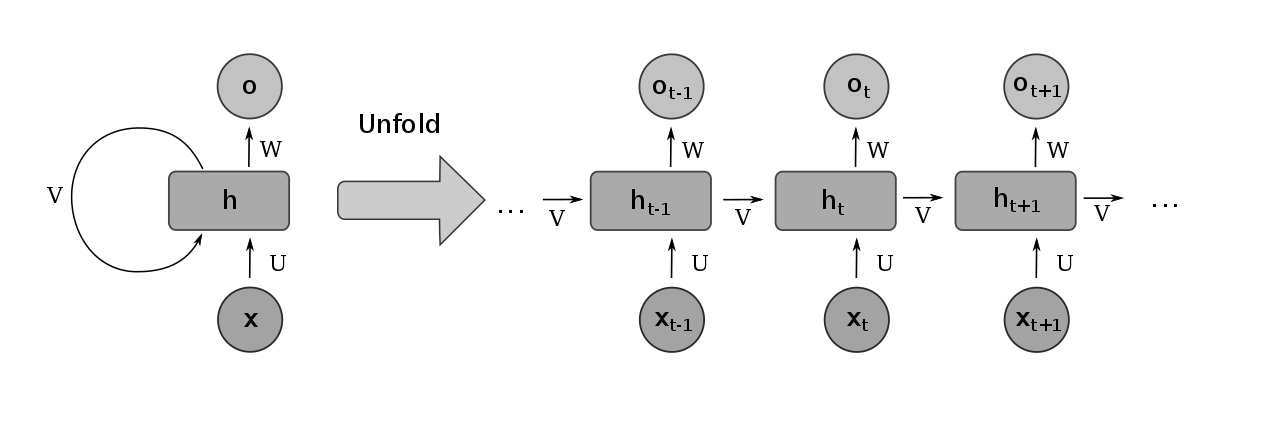
\includegraphics[width=0.6\paperwidth]{img/rnn_unfold.png}}
		\caption{A single-unit recurrent neural network and the unfolding in time of its computations \cite{WikipediaRNNunfold}.}
	\end{figure}
\end{center}

\subsection{Evaluate neural networks} \label{Evaluate neural networks}
To evaluate the networks' performances on a classification task, it's helpful to know how a \textit{confusion matrix} works: given a positive pattern, it can be correctly classified as positive, or misclassified as negative. These predictions are respectively called True Positive (TP) and False Negative (FN). The opposite happens when the pattern is negative, where the correct prediction is called True Negative (TN), and the wrong one is called False Positive (FP). The actual classification and the predicted one make up the columns and the rows of the confusion matrix.

\begin{table}[ht!]
	\centering
	\begin{tabular}{cccc}
									 &                            & \multicolumn{2}{c}{\textbf{Predicted}} \\
									 & \multicolumn{1}{c|}{}      & True               & False             \\ \cline{2-4} 
	\multirow{2}{*}{\textbf{Actual}} & \multicolumn{1}{c|}{True}  & True Positive      & False Negative    \\
									 & \multicolumn{1}{c|}{False} & False Positive     & True Negative    
	\end{tabular}
	\caption{Confusion matrix.}
\end{table}
Now some metrics are needed:
\begin{itemize}
	\item \textit{Accuracy}: the ratio of the correct classifications to the total observed cases. $\frac{TP+TN}{TP+FP+TN+FN}$
	\item \textit{Precision}: the ratio of the correctly identified positive cases from all the predicted positive cases. High precision means few false positives. $\frac{TP}{TP+FP}$
	\item \textit{Recall}: the ratio of the correctly identified positive cases from all the actual positive cases. High recall means few false negatives. $\frac{TP}{TP+FN}$
	\item \textit{F1 score}: the weighted average of precision and recall; gives a better measure of the incorrectly classified cases than the accuracy \cite{Hui19}. $2\, \frac{Precision \times Recall}{Precision + Recall}$
\end{itemize}

	\newpage
	\section{Technologies}

	\newpage
	\chapter{Development}
The goal of this chapter is to illustrate the new implementations and changes to the project's software, describing the improvements of the previous features, the new ones and the way in which they have been achieved.
\bigbreak

In the previous project's code, some time and memory optimizations have been made, minor bugs have been found and fixed and some other improvements have been done (e.g. replacing deprecated methods and libraries with newer ones).

\section{MQTT QoS2 caching}
As mentioned in the \textit{Unsolved Issues} chapter of Dario Piotrowicz's thesis \cite{Pio19}, there was a problem with unreliable Wi-Fi networks (an issue in the library's GitHub repository is still open \cite{githubQos2Issue}): all messages generated while a broken client-broker connection were discarded, instead of being stored to be sent when the connection will be re-established.

To solve that issue have been implemented two caching queues, one for each connection: the playing session one and the neural network's pattern collection one.

The cache size has been set to a safe value of 32 kilobytes (tested experimentally: bigger values led the Photon out of memory more often than not). The maximum number of messages that can be cached is stored in the \texttt{cache\_size} variable. With a maximum message size of 512 characters (511 effective characters because of the null terminator), the value is easily calculated as 32.

The following is a graph of the playing session's connection caching implementation; the neural network one is analogous.
\bigbreak

\begin{lstlisting}[style=CPPStyle]

	...

	// ready to send the data (publishString) to the client
	if (client.isConnected()) {
        while (cached_messages.size() > 0) {
			// send cached messages
            std::string msg = cached_messages.front();
            cached_messages.pop();
			client.publish("motiontracker/" + ID,
							msg.c_str(),
							MQTT::QOS2);
        }
		client.publish("motiontracker/" + ID,
						publishString,
						MQTT::QOS2);
    } else if (cached_messages.size() < cache_bound) {
		// save message in cache
        std::string msg(publishString);
        cached_messages.push(msg);
    }

	...

\end{lstlisting}
\bigbreak

This solution has made possible to damper temporary disconnections caused by instable connections.

\section{Delay in real-time data plotting}
\dots

\section{Motion capture}
In the software's previous version, developed and improved by Dario Piotrowicz \cite{Pio19} from the Marco Lanini's project \cite{Lan17}, the data processed by the device and sent to the server were:
\begin{itemize}
	\item device's orientation both in quaternions and yaw, pitch and roll angles;
	\item device's acceleration in Cartesian and spherical coordinates system;
	\item raw accelerometer, gyroscope and magnetometer data;
	\item device's velocity approximation.
\end{itemize}

This work's aim is to detect \textit{discriminating features among different playing patterns}, by collecting and analyzing the sensors data stream; the analysis followed the flow in the data fusion schema (Figure \ref{old data fusion schema}), except for the velocity approximation.
\bigbreak

The velocity approximation, calculated by the \textit{Velocimeter} class \cite{Pio19}, was early excluded because of the practical difficulty in obtaining realistic values using only inertial sensors, where measurement errors are unavoidable, especially for miniature MEMS sensors \cite{Du15, Est14, Kow15, Liu01, Sei07, UsingAcc, Woo07, Yan06}.

Direct integration of acceleration often causes unrealistic drifts in velocity, due to errors propagation; furthermore, measured acceleration not only carries random noise, but also presents with offset caused by temperature drift \cite{Kow15, Liu01, Woo07}, resulting in estimation errors accumulated by integration process, that results in low accuracy.

In particular, two behaviors were miscalculated:
\begin{itemize}
	\item stillness after a movement: if the truck toy is pushed from behind and it is left to stop alone, the velocity is expected to linearly decrease down to zero, but the velocity graph shows an uniform-like decrease in the first phase, and a peak towards zero in the last one;
	\item repetitive light accelerations: the vertical acceleration generated by the tessellated tyres rolling resulted in absent vertical velocities.
\end{itemize}

\begin{center}
	\begin{figure}[ht]
		\makebox[\textwidth]{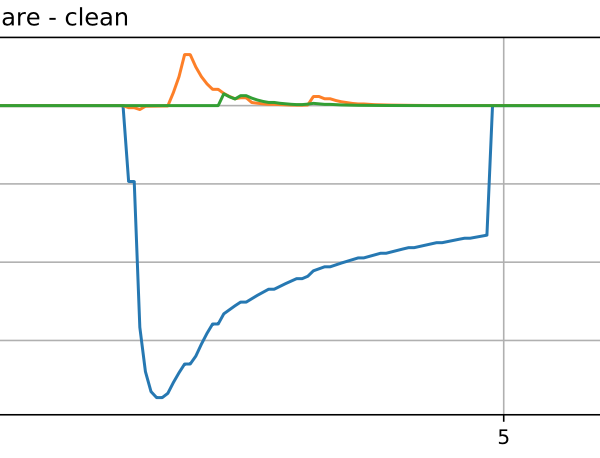
\includegraphics[width=0.2\paperwidth]{img/plots/square.png}}
		\caption{Square wave and absent velocities.}
	\end{figure}
\end{center}

\subsection{Gravity-affected data}
The first analytic phase dealt with raw accelerometer data, but the signal's noisiness and the presence of gravity have induced to desist. Nevertheless, especially for movements with strong accelerations, that simply increase the signal-to-noise ratio, the main waveform was recognizable.
\bigbreak

TODO: graph
\bigbreak

The analysis moved to Kalman-filtered data, which proved to be much cleaner and smoother, but still influenced by gravity; thus it would have been necessary a more complex training data collection, due to the lack of orientation invariance – the gravity decomposes among the axes in accordance with device's orientation, influences other accelerations, and affects the neural network's training: the neural network would believe that the gravity is part of the pattern acceleration; consequently, the same pattern recorded with a different device's orientation would be classified differently. To achieve such invariance it would be necessary to collect every pattern with the device rotated in any possible angle.
\bigbreak

TODO: graph
\bigbreak

Nevertheless, it was discovered that the gravity-free acceleration computed by the device and sent to the server was not stored in the database, but only used for the 3D visual representation. It was decided to store such data in the database along with other sensors data, and analyze it to see whether it was reliable over time. A smooth gravity-free acceleration could have been the turning point for an efficient neural network training and future classification.
\bigbreak

\subsection{Gravity-free data}
Analyzing gravity-free data, another problem showed up: after a few minutes of playing, the calculation of the yaw angle accumulated errors that led it to diverge in an unrealistic way, rotating counterclockwise, and consequently the accelerations no longer matched the device's orientation. The error didn't grow with the still device, but only when the device was moved, and therefore it should not be confused with the \textit{yaw drift} problem, that leads the yaw to rotate constantly in any device condition, and it's often caused by biases in gyroscope measurements (and that's the case of this project \cite{Pio19}) or poor/absent magnetometer calibration.
\bigbreak

The yaw's measurement was particularly affected by rotations around the Earth's $z$-axis (in other words, over the plane generated by the $x$ and $y$ axes), and the bigger the pitch angle, the bigger the error, as shown in the table below. Pitch and roll, on the contrary, were calculated almost without errors.
\bigbreak

\begin{table}[ht]
	\centering
	\begin{tabular}{c|c c}
	\textbf{Pitch} ($^{\circ}$) & \textbf{Mean error} ($^{\circ}$) & \textbf{Standard deviation} ($^{\circ}$) \\ \hline
	0                           & 47.12                            & 0.94                                     \\
	20                          & 47.67                            & 1.88                                     \\
	40                          & 51.14                            & 1.45                                     \\
	60                          & 58.14                            & 1.73                                     \\
	80                          & 57.80                            & 0.75
	\end{tabular}
	\caption{Yaw errors after a 360$^{\circ}$ rotation with different pitch angles.}
\end{table}

\begin{center}
	\begin{figure}[ht]
		\makebox[\textwidth]{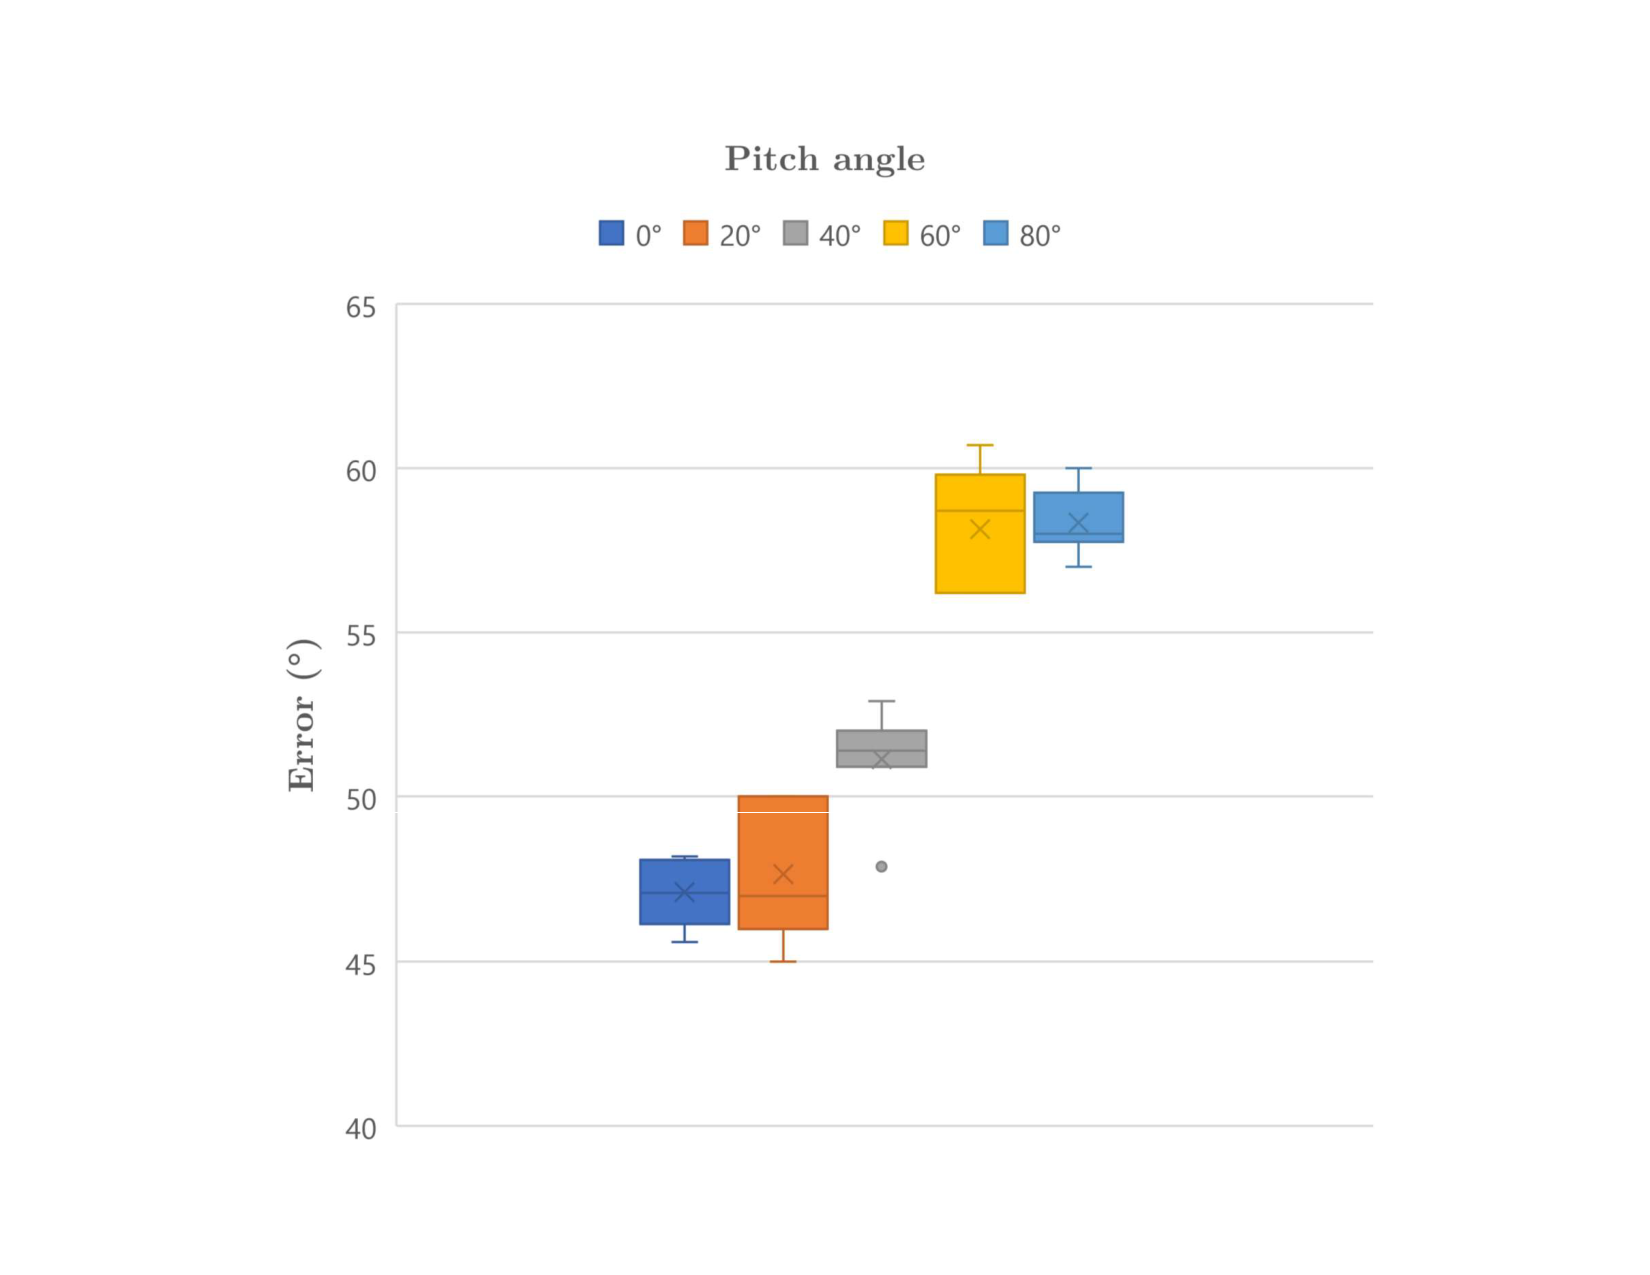
\includegraphics[width=0.55\paperwidth]{img/yaw_errors.pdf}}
		\caption{Box plot of yaw errors.}
	\end{figure}
\end{center}

Small yaw variations were also noticed with pitch-only movements: after a 360$^{\circ}$ rotation, the mean error was 0.47$^{\circ}$ with a standard deviation of 0.11$^{\circ}$.

\begin{center}
	\begin{figure}[ht]
		\makebox[\textwidth]{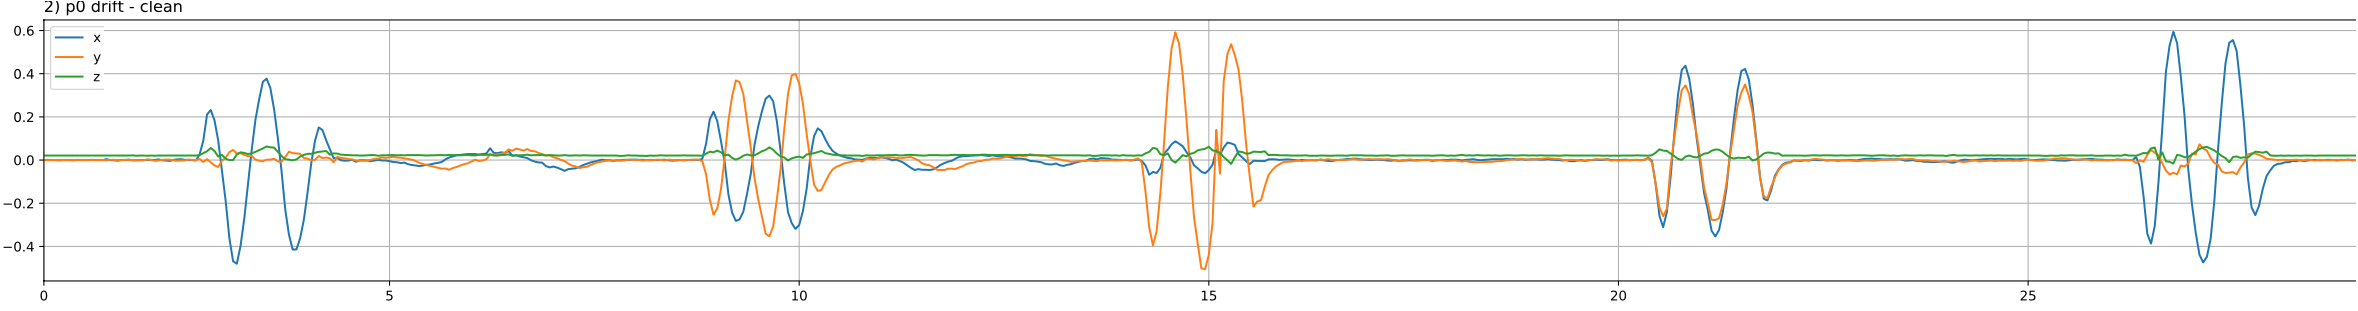
\includegraphics[width=0.7\paperwidth]{img/plots/drift.png}}
		\caption{Different accelerations for the same pattern.}
	\end{figure}
\end{center}

During some tests, it was noticed another unexpected behavior: different recordings of the same pattern with different device rotations showed the same acceleration among axes (e.g. given a fixed three-dimensional path, following it with the truck facing forwards, backward, upside-down or other, would show exactly the same accelerations).
\bigbreak

TODO: Plot with the same movement with different orientations that shows the same data
\bigbreak

The cause of the error was discovered to be in the Madgwick's algorithm implementation, more precisely in the lack of yaw's convergence in its error-correction gradient descent phase (see section \ref{Madgwick filter}). Unfortunately, several algorithm implementations that included the correction, and different values of the algorithm's gain parameter (the magnitude $\beta$ of the gyroscope measurement error\footnote{Increasing $\beta$ leads to faster bias corrections and higher sensitiveness to lateral accelerations.} \cite[13]{Mad10}) gave no better results over time, and worse, ghost accelerations were found. Then, the Lanini's version has been kept and the troubleshooting continued.
\bigbreak

Since the accelerations were independent from the orientation of the device, the cause was necessarily the reference system's location, which proved to be global: the movements were shown as viewed by an external observer, placed in the Earth's center.

To align the reference system back, it was sufficient to rotate the acceleration vector by the 3 orientation angles (of \textit{yaw}, \textit{pitch} and \textit{roll}) given by the Madgwick's algorithm, and that, as shown below, not only correctly brought the reference system back to a local point of view, but surprisingly solved the yaw alignment issue.

The explanation of this (apparent) side-effect lies in how the gravity subtraction is performed: as shown in the Figure \ref{old data fusion schema}, the data obtained from the Kalman and Madgwick filters are used jointly. As discussed above, the Kalman filter does not present any problem, while the Madgwick one fails in the yaw angle calculation; hence, the resulting acceleration is misaligned, and needs to be corrected by the same misalignment angle: the Madgwick's angle itself.
\bigbreak

The rotation of the acceleration vector has been performed through a three-dimensional rotation matrix. In three-dimensional matrices, the matrix-vector multiplication doesn't affect the speed meaningfully, even for relatively weak CPUs like the one that runs in the Photon: the goal packets' frequency of 22 Hertz \cite{Pio19} has been always achieved (when the wireless connection allowed it) and however the C++ code is compiled by \texttt{GCC} with the \texttt{-Os} flag, that includes the loop unrolling optimization \cite{UsingGCC}.

\begin{center}
	\begin{figure}[ht]
		\makebox[\textwidth]{
\includegraphics[width=0.7\paperwidth]{img/plots/nodrift.png}}
		\caption{Image of correct accelerations.}
	\end{figure}
\end{center}

\subsection{Fine tuning: magnetic distortions}
Once achieved a reliable gravity-filtered acceleration approximation, it was possible to perform some fine tuning.
\bigbreak

It is known that magnetic and inertial sensors can be influenced by magnetic disturbance \cite{Fan17}.
There are two types of magnetic distortions:
\begin{enumerate}
	\item \textit{soft iron}: it's a temporary influence that appears when a material is affected by the Earth's magnetic field, and it's induced from metals that are non permanently magnetised (they don't generate a magnetic field themselves) \cite{Cro15}. It causes errors in the measured direction of the Earth's magnetic field, and since it depends on the orientation of the material relative to the sensor and the magnetic field, it cannot be compensated by a constant \cite{CompensatingIron};
	\item \textit{hard iron}: it's produced by materials that exhibit a constant, additive field to the Earth's magnetic field \cite{CompensatingIron}, and it can be simply removed by a constant offset, calculated through calibration \cite{CompensatingIron, Geb06, Kok12}.
\end{enumerate}

Madgwick's algorithm is able to remove \textit{soft iron} distortions \cite[11-12]{Mad10}, and the calibration to remove \textit{hard iron} distortions has been performed by the SparkFun's Arduino library.
\bigbreak

Unfortunately, there are non-constant interferences that still affect the sensors readings, such as the magnetic field generated by the current passing through the USB cable for charging the battery.
Its removal is much harder, because requires to analyze how much current is flowing through the cable, and the knowledge of the net magnetic field's shape, that depends on how the cable is placed around the sensor.

\begin{center}
	\begin{figure}[ht]
		\makebox[\textwidth]{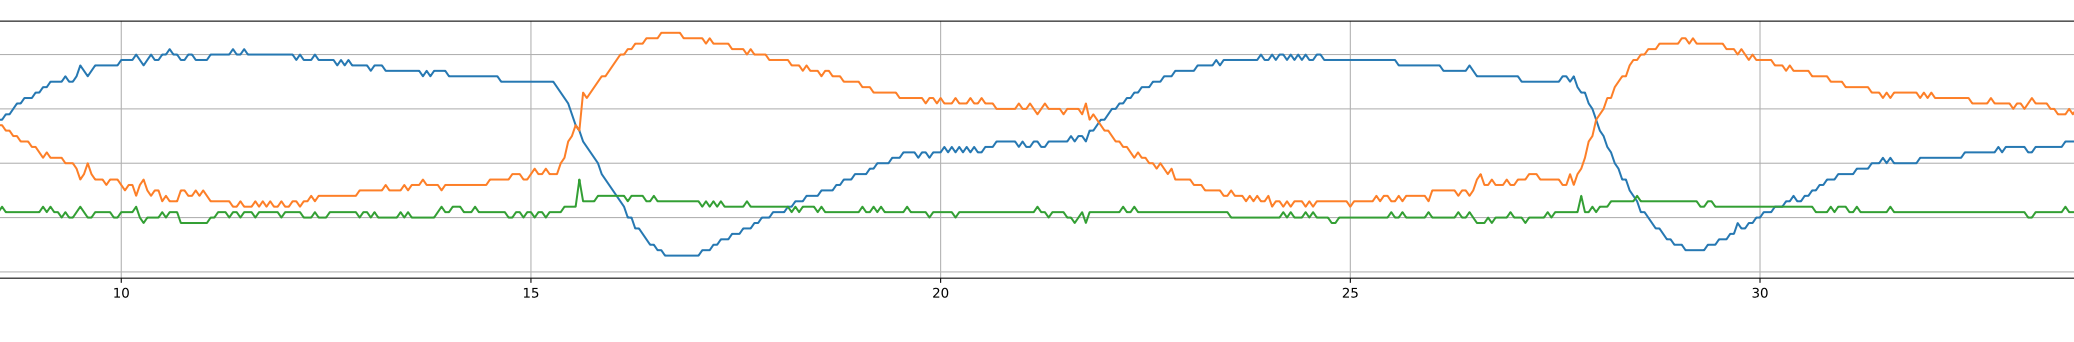
\includegraphics[width=0.7\paperwidth]{img/plots/battery.png}}
		\caption{Orientation affected by the battery charging.}
	\end{figure}
\end{center}

\subsection{Final data fusion schema}
The current data flow is illustrated by the schema:

\begin{center}
	\begin{figure}[ht]
		\makebox[\textwidth]{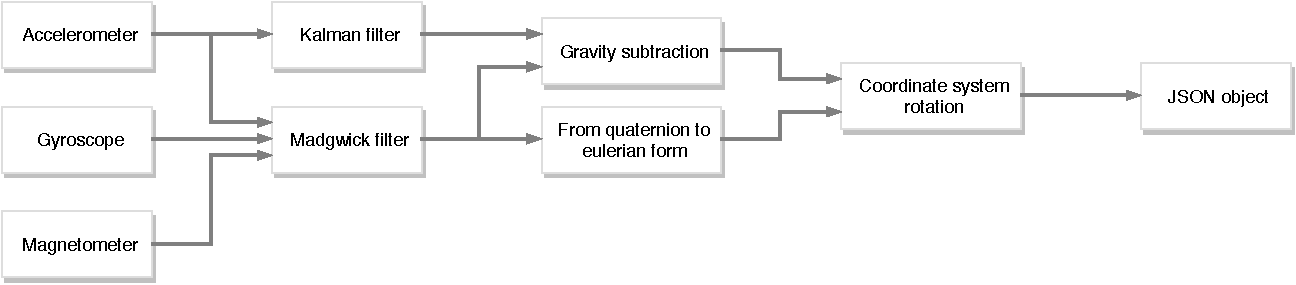
\includegraphics[width=0.65\paperwidth]{img/data_fusion.pdf}}
		\caption{Current data fusion schema.}
	\end{figure}
\end{center}

\subsection{Smart pattern recording}
Previously, the recording of a pattern for the training set was simply triggered by specific buttons in the web page, that once pressed, started immediately the recording. Since the recording time was quite short (500ms), it was difficult to start moving the toy exactly when the server started recording, because the movement could start too early or too late: both can cause data loss, but the second case is subtly more dangerous, including movements unrelated to the pattern inside the recording.

To prevent unintended movements from being saved, the recording module was modified in this way: the buttons no more trigger the immediate start of the recording, but sends the server in a \textit{waiting} state, an intermediate state where it asynchronously waits the toy to being moved. When the toy is moved, the real recording starts, without any data loss.

The motion detection is performed by the toy itself, and sent to the server through an attribute in the JSON object; unfortunately it has been found a slight delay between the real movement and its detection, empirically measured as 150ms, that corresponds to 3 packets, sent by the device but discarded by the server: to solve this problem, a small buffer has been included within the recording module, and these packets are punt in front of the ones that would be saved before.

\begin{center}
	\begin{figure}[ht]
		\makebox[\textwidth]{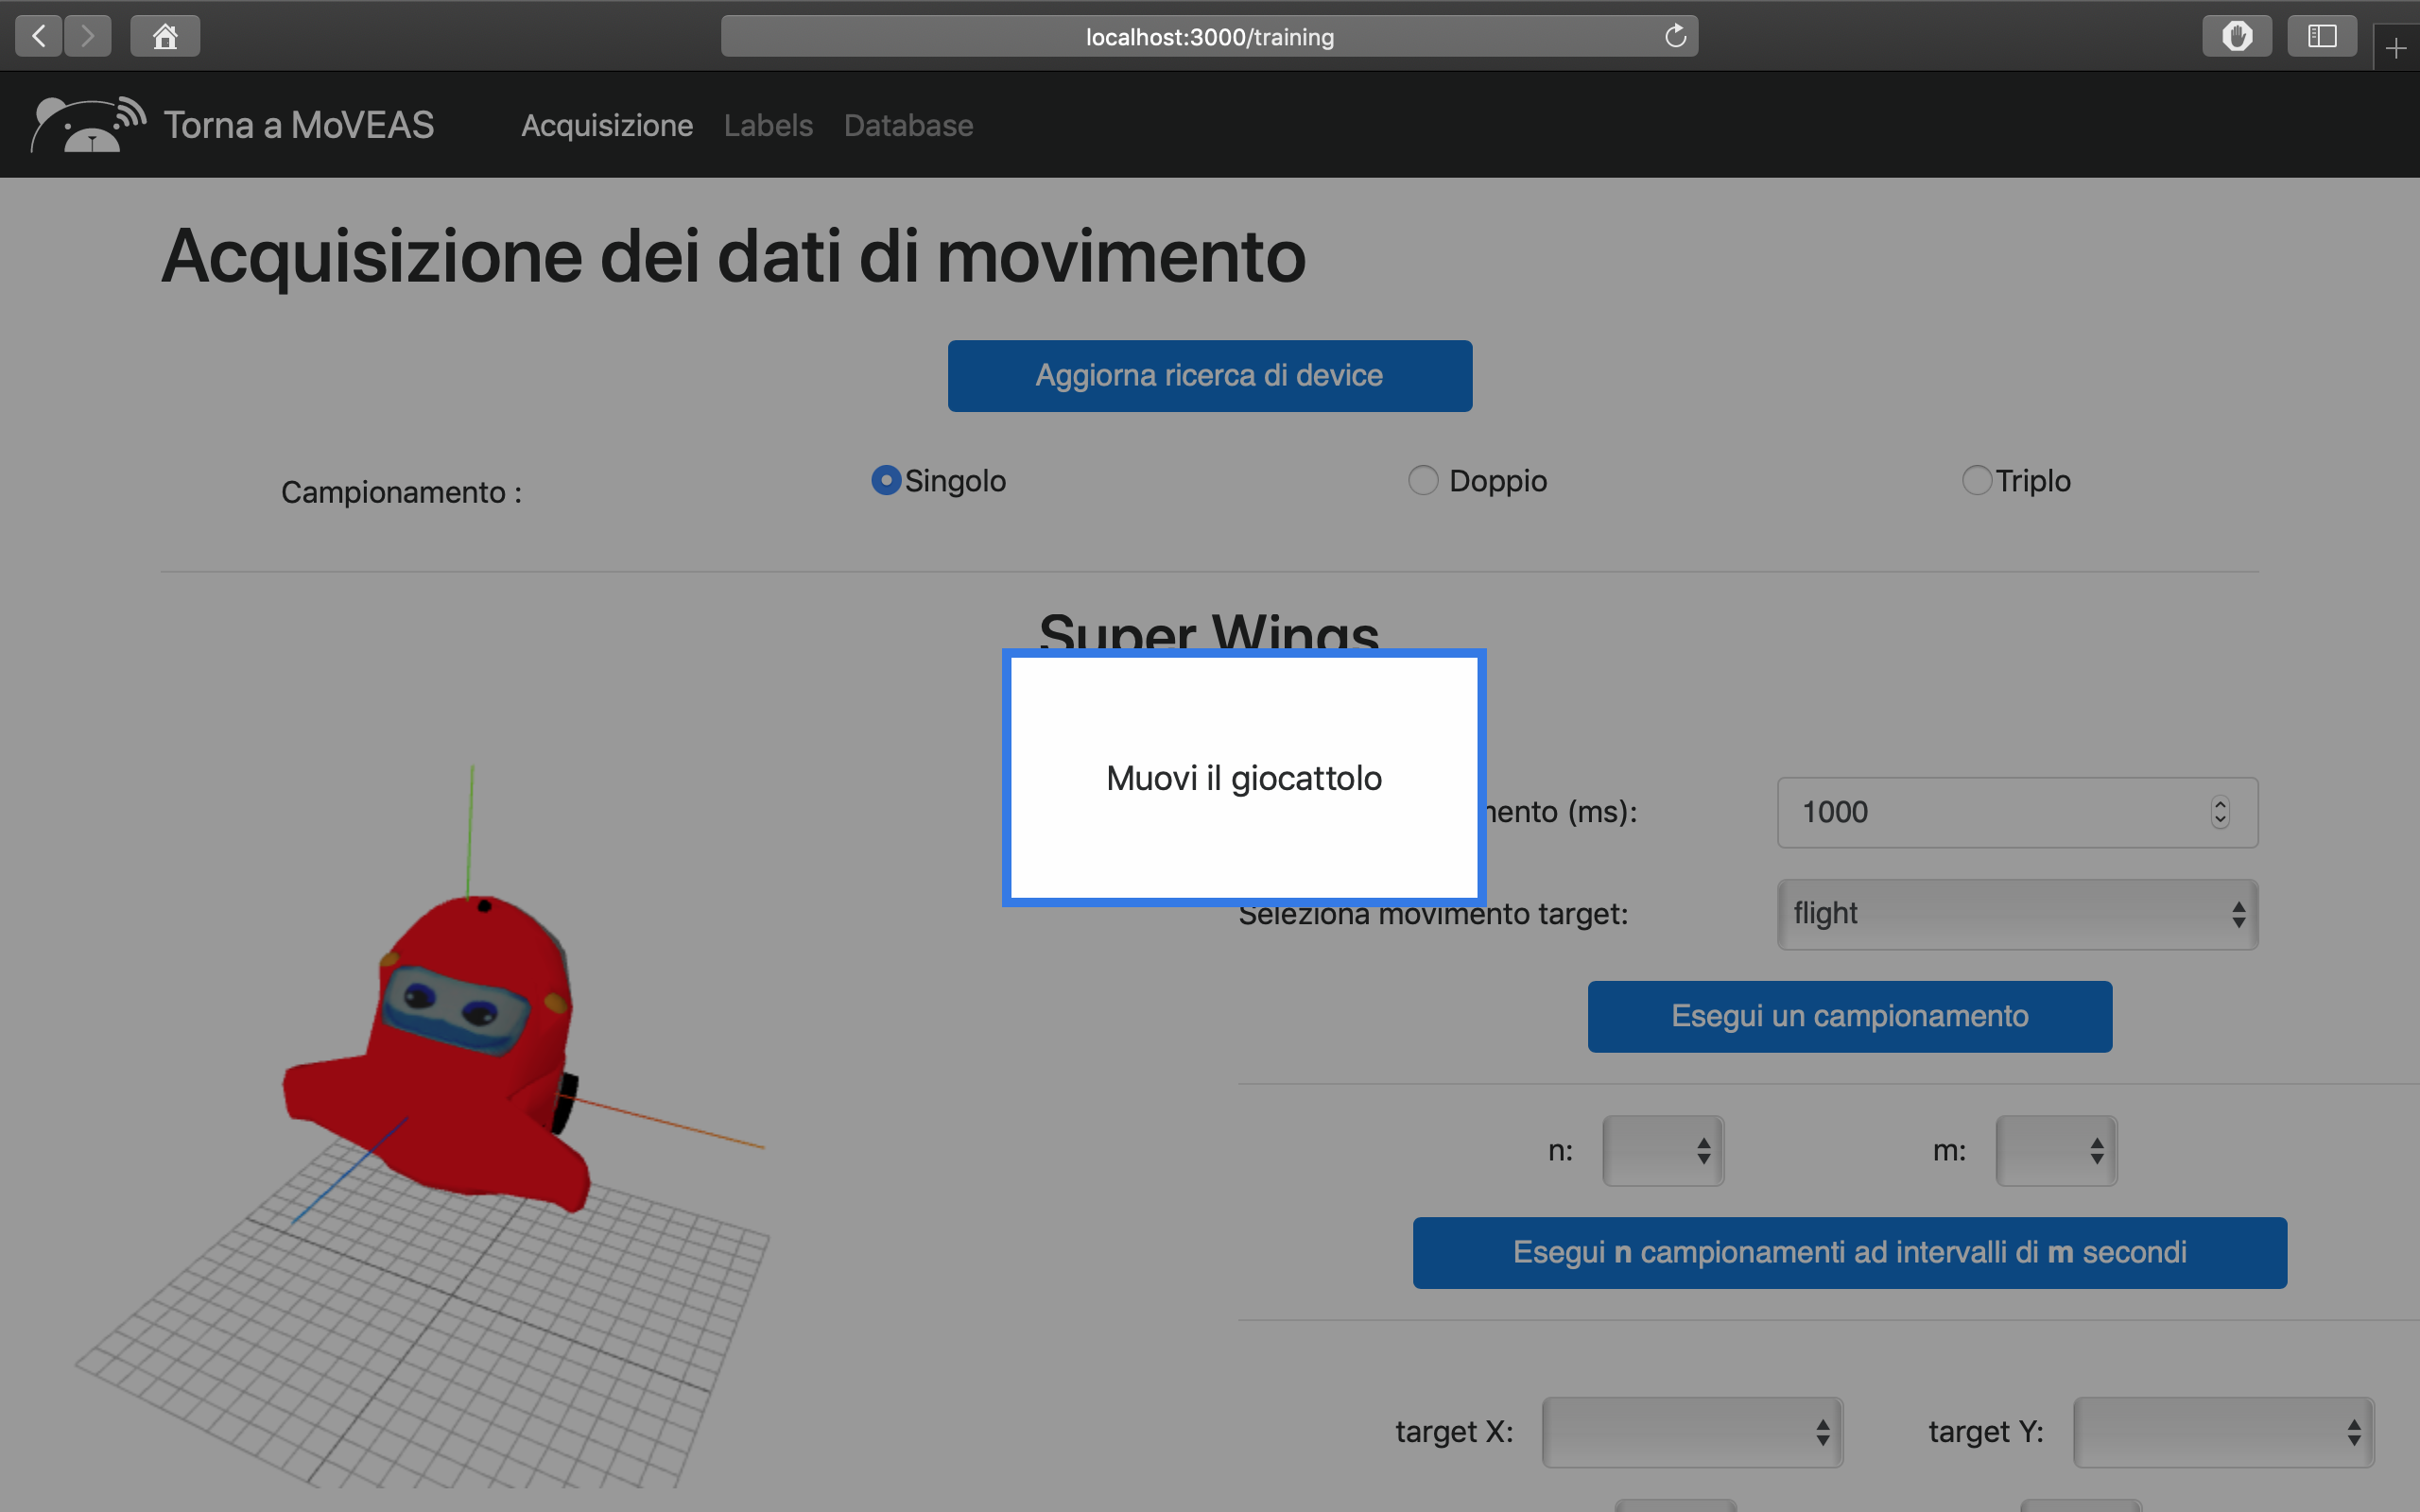
\includegraphics[width=0.6\paperwidth]{img/wait.png}}
		\caption{The recording module the waiting state.}
	\end{figure}
\end{center}
Not all patterns need the same recording time: for example, the movement of the toy pushed forward is much smaller than the one where the toy is thrown against a pillow, where the toy is thrown by the hand first, then flies in the air until it reaches the pillow. To adapt the module to this eventuality, it has been added the possibility to change the duration of the recording. Nevertheless, not every neural network can deal with variable-length sequences.

\section{Time series classification}
Standard feedforward neural networks are not suitable for time series classification tasks, because they are not \textit{shift-invariant} (in this case, time-invariant). For time series patterns, this allows the network to classify a pattern regardless of its start time.

\subsection{Dataset}
For model training and validation, the dataset was composed of:
\begin{itemize}
	\item 100 patterns with the toy going \textit{forward} and 100 with the toy going \textit{backward};
	\item 200 patterns of simulated \textit{flight};
	\item 200 patterns with the \textit{still} toy;
	\item 200 patterns of the toy carried while \textit{walking};
	\item 200 patterns of the toy \textit{thrown} against a pillow.
\end{itemize}
The training and validation portions were respectively the 60\% and the 40\% of the total, and the entire dataset is shuffled before every training.

The test set was composed of 240 samples, disjoint from the training and validation ones.
\bigbreak

In this work, two network's models have been chosen, and their performance compared. The first one is a time delay neural network, chosen for its simplicity, since the training sequences were short (22 samples) and a complex model might go very easily to overfitting; the second one is a recurrent neural network, chosen for its ability to recognize variable-length patterns.

The following part explains how the model selection was done.
\bigbreak

\subsection{Time delay neural network}
\subsubsection{Topology and activation functions}
The model selection started from the simplest topology: an input layer with data normalization, a convolutional hidden layer with a \textit{ReLU} activation function, that performed better than \textit{tanh}, and an output layer for the pattern classification, with a \textit{softmax} function, to obtain values between 0 and 1, representing the probability of the classified pattern to belong to each possible class.
\bigbreak

\begin{center}
	\begin{figure}[ht]
		\makebox[\textwidth]{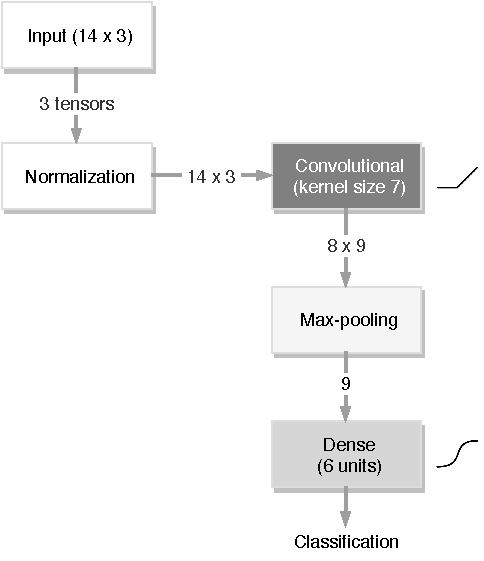
\includegraphics[width=0.35\paperwidth]{img/tdnn_topology.pdf}}
		\caption{TDNN final topology.}
	\end{figure}
\end{center}

\subsubsection{Features}
Only three features were considered relevant for the training: the gravity-free accelerations values in the three axes. Some tests showed quickly that adding more features, like orientation, velocity data, or raw sensors data, made the network almost untrainable with this simple model.

\subsubsection{Hyperparameters}
The search for the two most important hyperparameters, the \textit{kernel} size and the number of \textit{filters}, has been performed through a \textit{grid search}. For each table's entry, the network has been tested 10 times, with shuffled data between testing and validation set for each run. Outliers have been omitted from the average.

\begin{table}[ht]
	\centering
	\begin{tabular}{cccccc}
									  &                         & \multicolumn{4}{c}{\textbf{Kernel size}} \\
									  & \multicolumn{1}{c|}{}   & 3        & 5        & 7        & 9       \\ \cline{2-6} 
	\multirow{7}{*}{\textbf{Filters}} & \multicolumn{1}{c|}{3}  & 90,00\%  & 92,57\%  & 95,00\%  & 98,25\% \\
									  & \multicolumn{1}{c|}{5}  & 94,50\%  & 95,50\%  & 98,50\%  & 99,00\% \\
									  & \multicolumn{1}{c|}{7}  & 98,80\%  & 99,00\%  & 99,87\%  & 99,90\% \\
									  & \multicolumn{1}{c|}{9}  & 97,93\%  & 99,00\%  & 99,65\%  & 99,87\% \\
									  & \multicolumn{1}{c|}{11} & 98,06\%  & 98,52\%  & 99,59\%  & 99,83\% \\
									  & \multicolumn{1}{c|}{13} & 96,94\%  & 99,53\%  & 99,91\%  & 99,84\% \\
									  & \multicolumn{1}{c|}{15} & 99,20\%  & 99,88\%  & 99,90\%  & 99,90\%
	\end{tabular}
	\caption{Average training accuracy.}
\end{table}

\begin{table}[ht]
	\centering
	\begin{tabular}{cccccc}
									  &                         & \multicolumn{4}{c}{\textbf{Kernel size}}       \\
									  & \multicolumn{1}{c|}{}   & 3       & 5       & 7            & 9           \\ \cline{2-6} 
	\multirow{7}{*}{\textbf{Filters}} & \multicolumn{1}{c|}{3}  & 77,68\% & 81,50\% & 92,33\%      & 87,33\%     \\
								      & \multicolumn{1}{c|}{5}  & 87,17\% & 92,73\% & 95,25\%      & 94,53\%     \\
									  & \multicolumn{1}{c|}{7}  & 90,38\% & 97,92\% & 95,68\%      & 95,25\%     \\
									  & \multicolumn{1}{c|}{9}  & 95,50\% & 97,29\% & 98,00\%      & overfitting \\
									  & \multicolumn{1}{c|}{11} & 94,60\% & 96,50\% & 97,75\%      & overfitting \\
									  & \multicolumn{1}{c|}{13} & 91,80\% & 93,50\% & 95,25\%      & overfitting \\
									  & \multicolumn{1}{c|}{15} & 93,00\% & 95,50\% & overfitting  & overfitting
	\end{tabular}
	\caption{Average validation accuracy.}
\end{table}
As shown in the tables, 9 and 7 were optimal values respectively for the number of filters and the kernel size: they gave the best result in the validation set, and in particular:
\begin{itemize}
	\item a number of filters up to 7 and a kernel size up to 5, made the network able to classify correctly only after a long and unstable training;
	\item from 7 filters upwards, the training curve was stable, and the overfitting occurred only from 15;
	\item kernel sizes from 9 upwards tended to overfit the network: the patterns were initially made of 22 samples, and the sliding window was be too big;
	\item with filters bigger than 20, the overfitting was mitigable only with very low kernel sizes, but in that case the network was hard to train, and very easy to underfit.
\end{itemize}
More complex topologies were tried, but adding hidden layers only led the neural network to the overfitting. The best training curve was obtained using 16-patterns long mini-batch.

According to \cite{Hin12}, dropout layers have not been added in the network.

\begin{center}
	\begin{figure}[ht]
		\makebox[\textwidth]{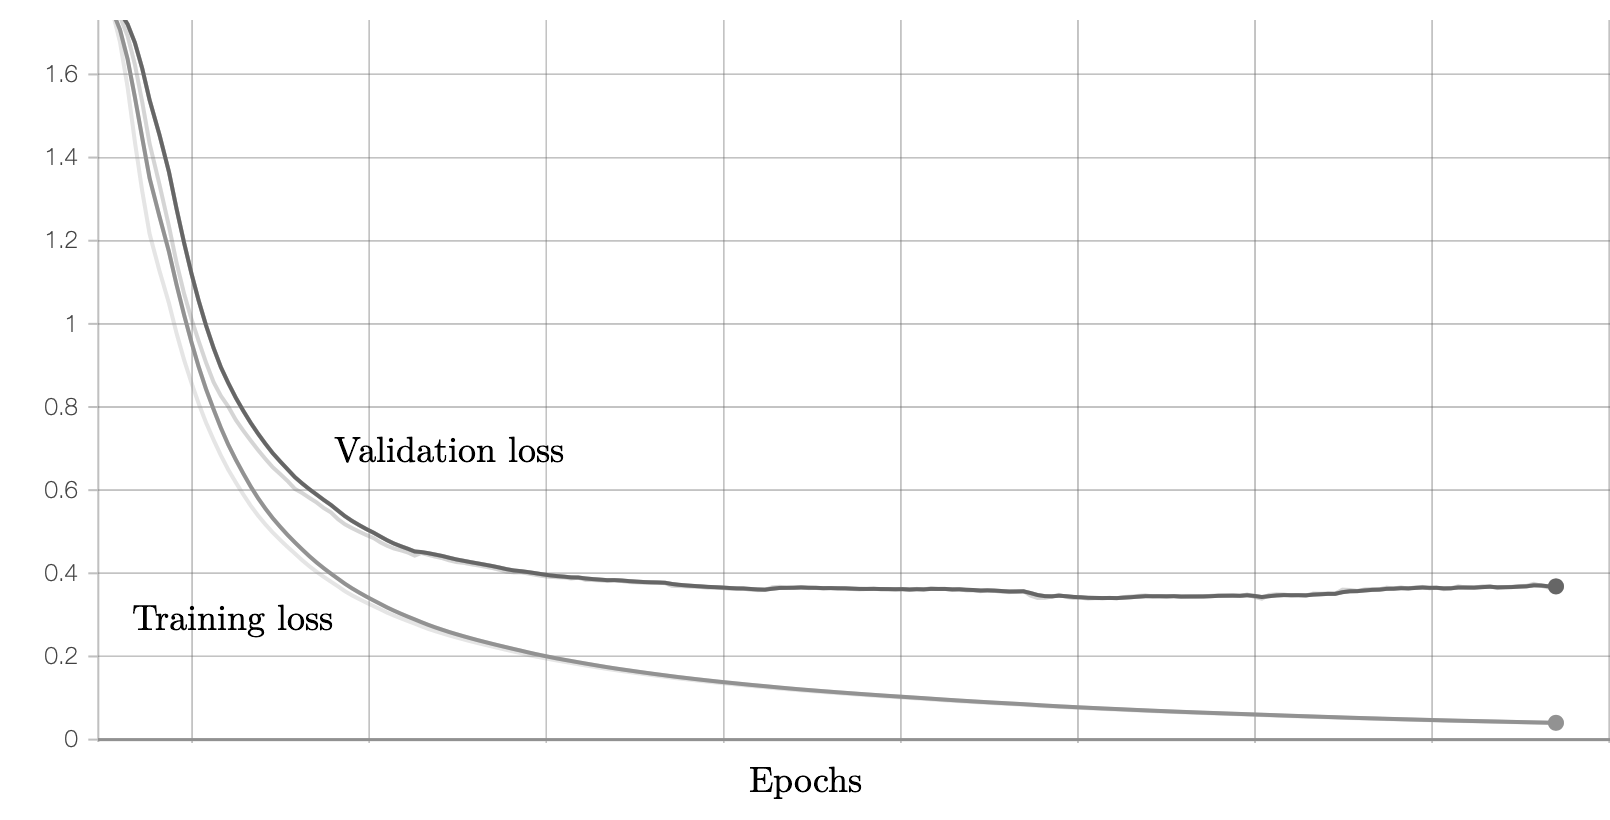
\includegraphics[width=0.65\paperwidth]{img/overfitting.png}}
		\caption{Overfitting due to high kernel size.}
	\end{figure}
\end{center}

\begin{center}
	\begin{figure}[ht]
		\makebox[\textwidth]{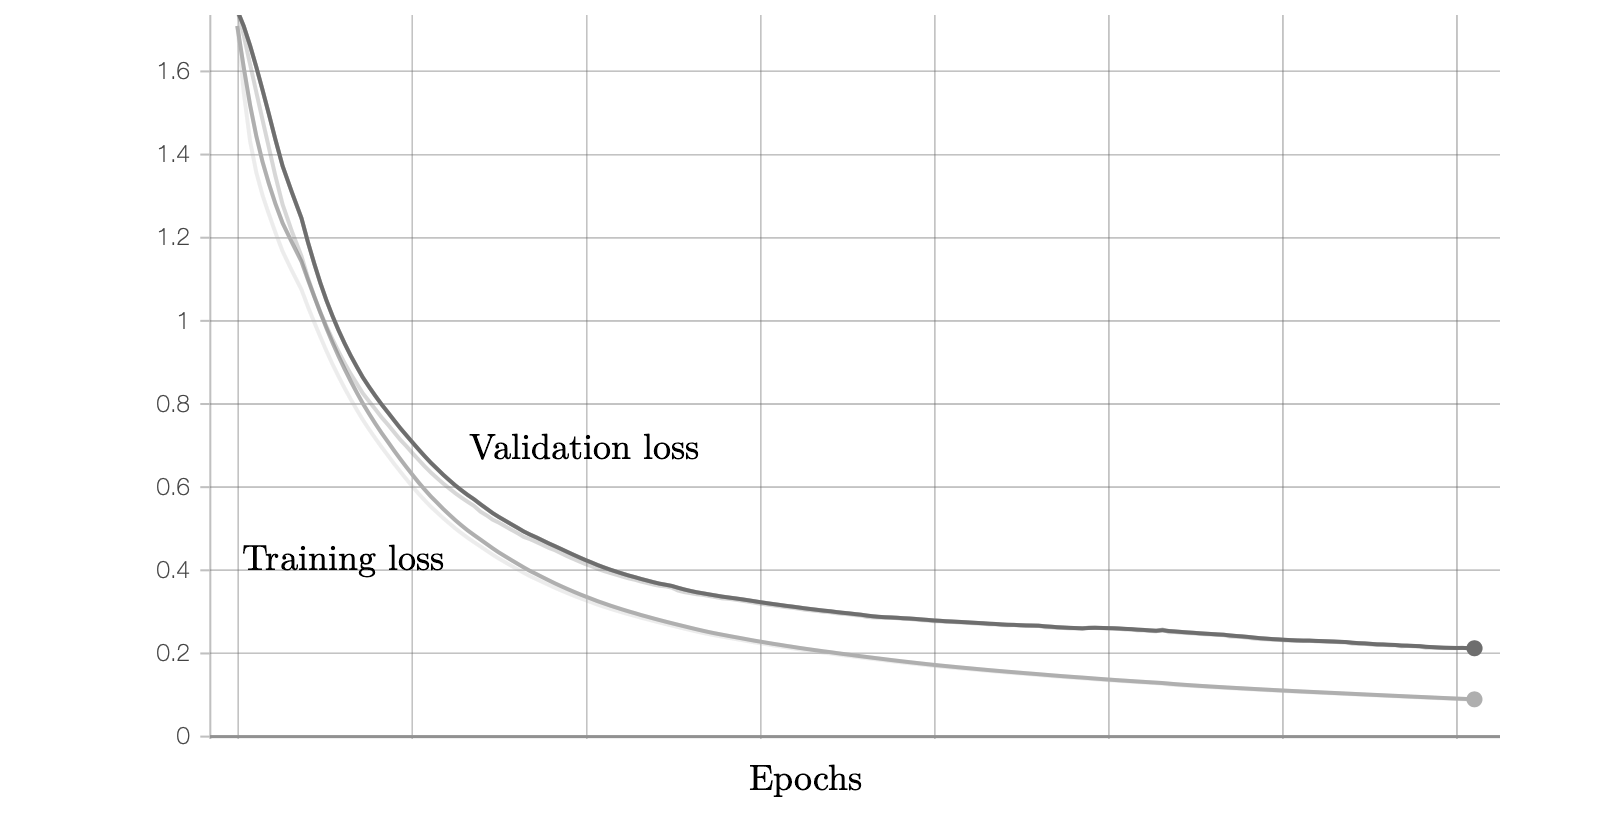
\includegraphics[width=0.65\paperwidth]{img/fitting.png}}
		\caption{Good fitting.}
	\end{figure}
\end{center}

\subsubsection{More accuracy with less data}
The next step was to achieve the maximum accuracy with less possible data. The network was trained several times with different patterns' lengths, and the best choice for a stable and accurate training has proved to be 15 samples per pattern, that with the 22 Hertz sampling means 682 milliseconds long patterns. Up to 11-13 samples, the network was not able to achieve good performance in training, being hard to train and underfitting, while from 17 samples and more, the network fitted the noise, so overfitted.

\begin{center}
	\begin{figure}[ht]
		\makebox[\textwidth]{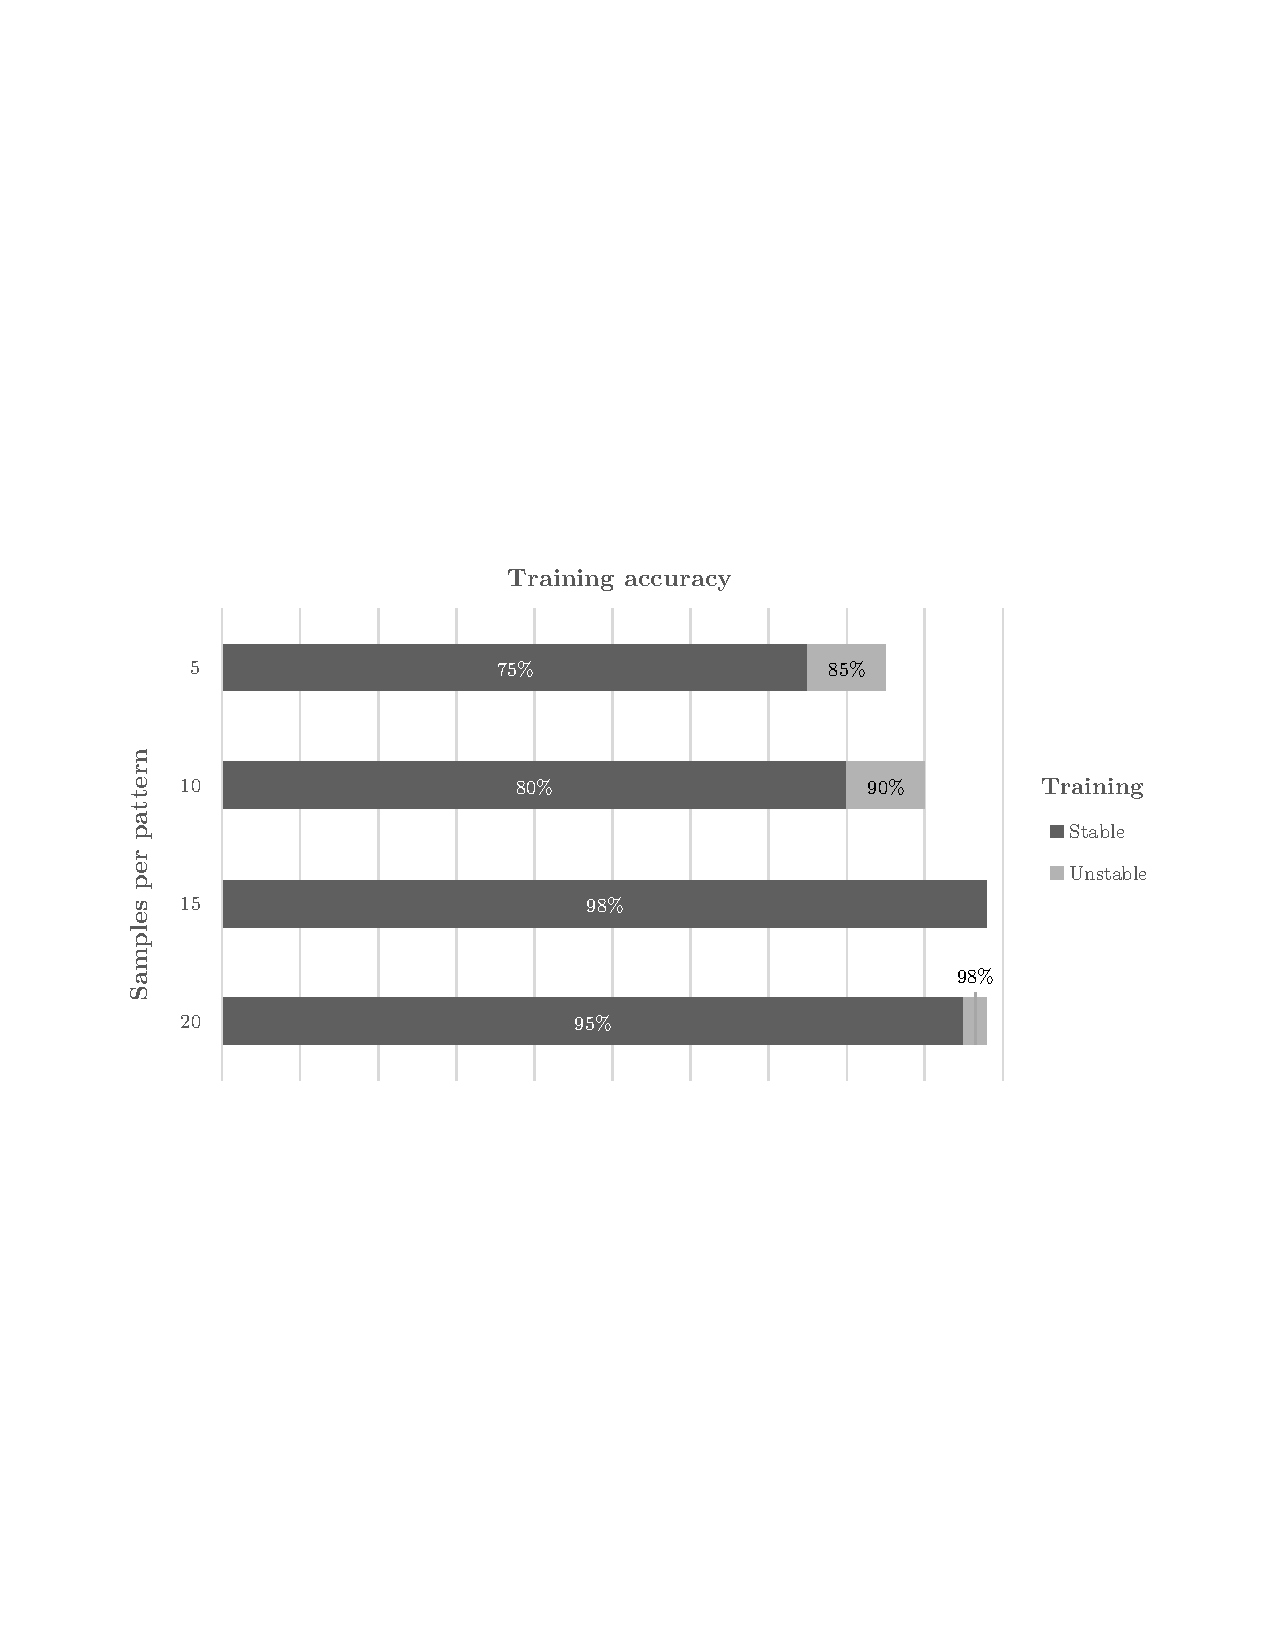
\includegraphics[width=0.65\paperwidth]{img/training_acc_samples.pdf}}
		\caption{Training accuracy with pattern with different lengths.}
	\end{figure}
\end{center}

\subsubsection{Regularization and optimization algorithms}
The convolutional layer's weights are initialized randomly in the uniform range [-0.000001, 0.000001]. To keep under control the network complexity, a \textit{weight decay} approach has been used, with tested values in the range [0.001, 0.05].
\bigbreak

TODO: Why adam optimizer? (paper) Batch size? (useless?)

\subsection{Recurrent neural network}
\subsubsection{Topology, activation functions and hyperparameters}
As done with the TDNN, the input passes through a normalization layer before going to the recurrent layer, and the activation function is \textit{ReLU} for all layers, except for the last one, that uses the \textit{softmax} function, particularly suitable for classification.
\bigbreak

The best topology, that ensured a good fitting without instabilities during the training, is shown in the following schema: one recurrent layer and two densely-connected layers, with two dropout layers before them. In particular, the number of nodes in the recurrent layer was crucial for the model selection:
\begin{itemize}
	\item up to 5 units, the network was able neither to learn the training samples nor generalize;
	\item up to 10 units, the validation accuracy reached almost the 90\%, but then overfitted;
	\item up to 12 units, the network was hard to train, and with 14 units the network was trained smoothly and the validation accuracy grew over 90\%;
	\item from 16 upwards, stricter regularization was needed, but the dropout layers made the training stable and avoided the overfitting. The best number of units was discovered to be 20.
\end{itemize}
The explored range of dropout for both layers was [0, 0.5]. The network was trained with a mini-batch size of 16.

\begin{center}
	\begin{figure}[ht]
		\makebox[\textwidth]{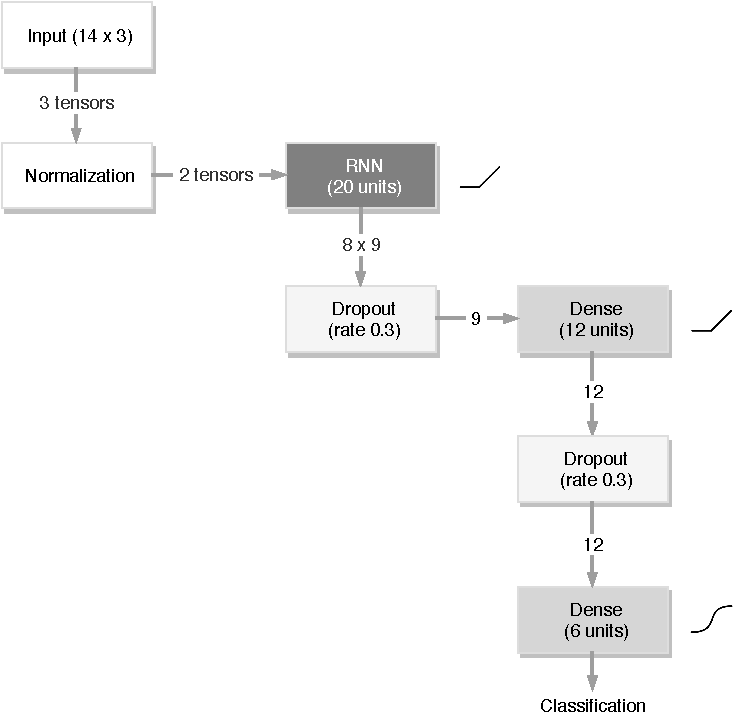
\includegraphics[width=0.55\paperwidth]{img/rnn.pdf}}
		\caption{RNN final topology.}
	\end{figure}
\end{center}

\subsubsection{Features and samples length}
Adding features besides the three acceleration values made the training harder and unstable, even with more layers and more recurrent units. 

In this model, reducing the number of samples has not improved the validation accuracy as for the TDNN, but the performance significantly decreased only for less than 14 samples per pattern, accordingly to the previous results.

\begin{center}
	\begin{figure}[ht]
		\makebox[\textwidth]{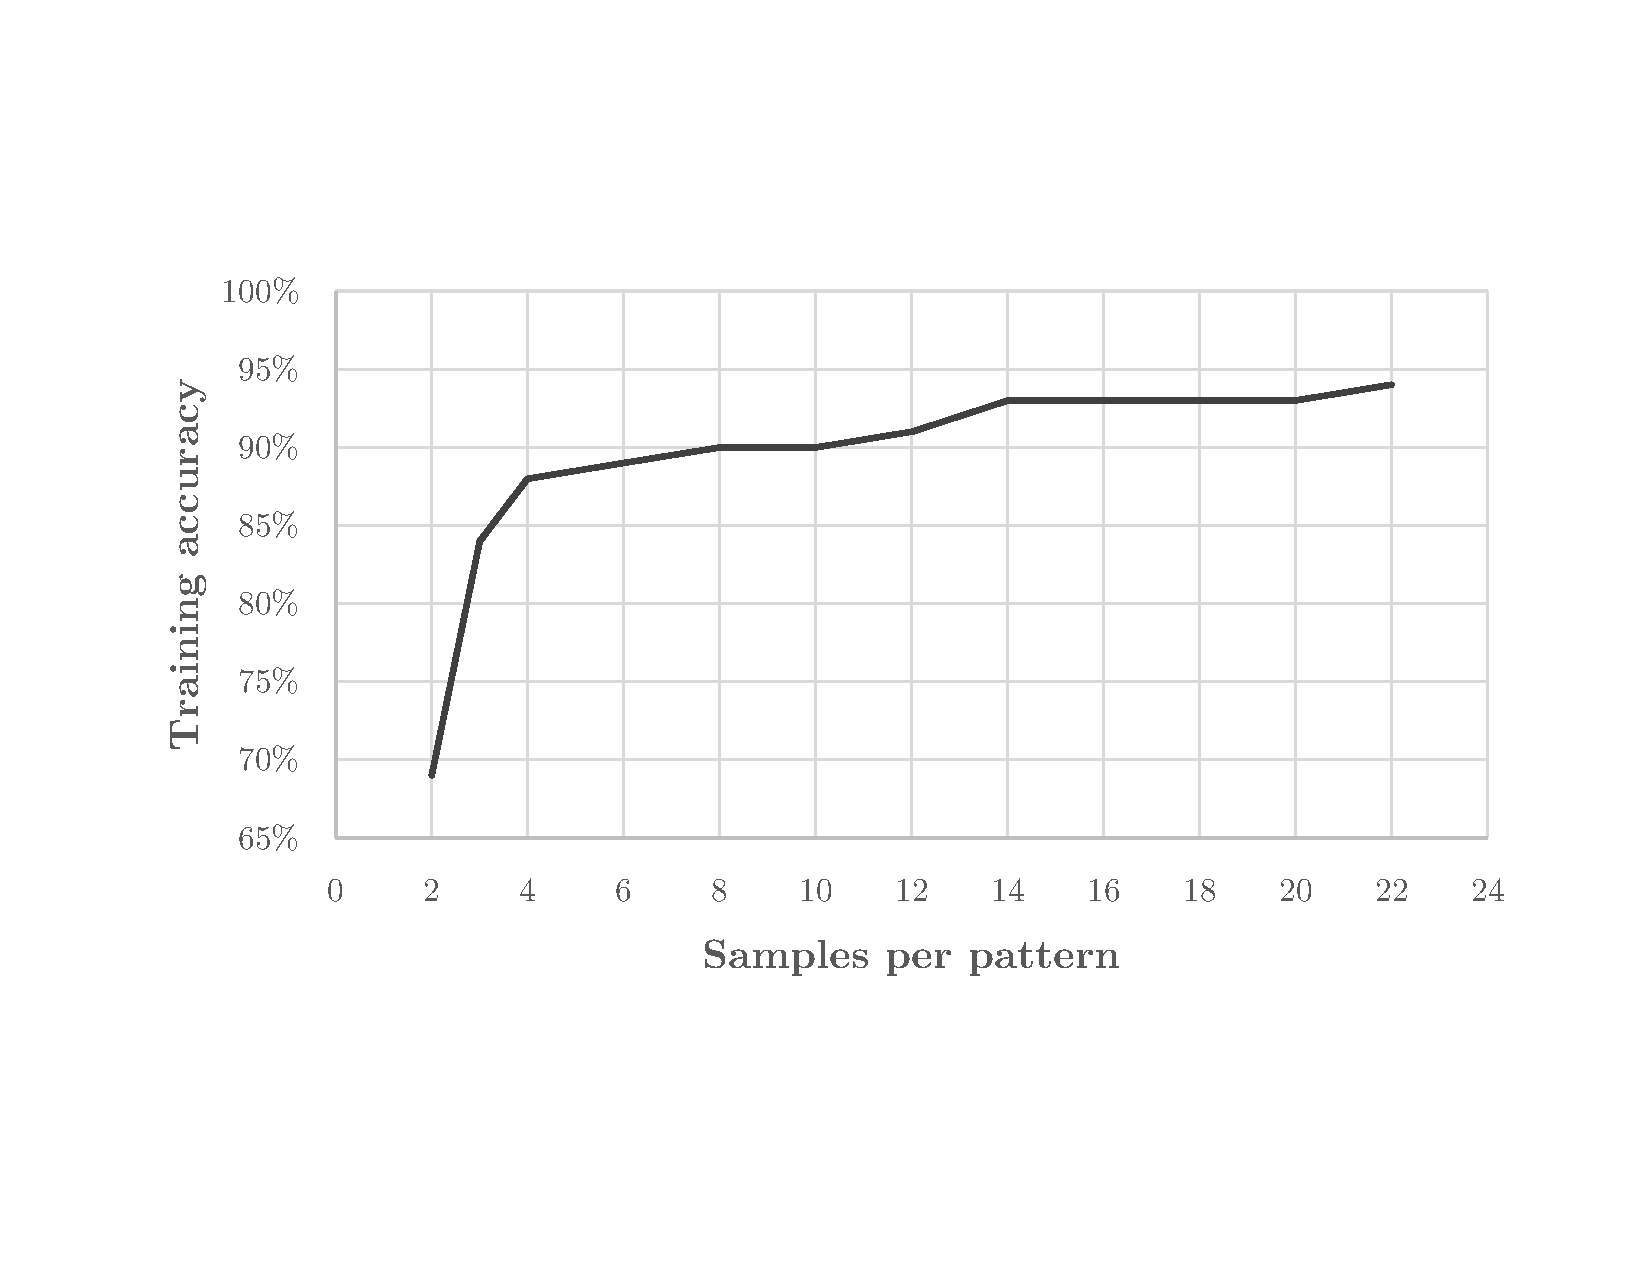
\includegraphics[width=0.6\paperwidth]{img/training_acc_samples_2.pdf}}
		\caption{\dots}
	\end{figure}
\end{center}

	\newpage
	\chapter{Conclusions}


	\printbibliography[nottype=online, title=Bibliography]
	\printbibliography[type=online, title=Sitography]

\end{document}
